\chapter{Gateway IoTs dựa trên nền tảng Android Things}
\label{chapter3}
\section{Tại sao phải cần hệ điều hành?}
"Để đạt được giá trị từ Internet of Things (IoT), việc cần phải có một nền tảng (platform) để tạo và quản lý ứng dụng, chạy các phân tích, lưu trữ và bảo mật dữ liệu của bạn là một điều cần thiết. Giống như một hệ điều hành dành cho máy tính xách tay, một nền tảng làm rất nhiều thứ đằng sau đó, giúp cho cuộc sống của các nhà phát triển, nhà quản lý và người dùng dễ dàng hơn và ít tốn kém hơn."\cite{tl4}

\subsection{Vậy nền tảng (platform) là gì?}
"Nói chung, nền tảng (platform) là phần mềm và phần cứng, có thể bao gồm môi trường hoạt động, lưu trữ, sức mạnh máy tính, bảo mật, công cụ phát triển và nhiều chức năng phổ biến khác. Nền tảng được thiết kế để hỗ trợ nhiều chương trình ứng dụng nhỏ hơn mà thực sự giải quyết các vấn đề kinh doanh.\\

Nền tảng hữu ích vì chúng rút ra rất nhiều chức năng chung từ logic ứng dụng cụ thể. Ví dụ, bất kể bạn đang cố gắng viết một ứng dụng để tối ưu hoá mức tiêu hao nhiên liệu hoặc không gian lớp học, cơ bản bạn cần khá nhiều công nghệ giống nhau. Các nhà phát triển ứng dụng chỉ muốn tập trung vào vấn đề cụ thể mà họ đang giải quyết và sử dụng các khả năng chung để tính toán sức mạnh hoặc lưu trữ hoặc bảo mật. Một nền tảng tốt làm giảm đáng kể chi phí phát triển và duy trì các ứng dụng.\\

Trong Internet of Things, các nền tảng được thiết kế để triển khai các ứng dụng giám sát, quản lý và kiểm soát các thiết bị được kết nối (hình bên dưới). Các nền tảng IoT phải xử lý các vấn đề như kết nối và trích xuất dữ liệu từ một số lượng khổng lồ các điểm cuối khác nhau, đôi khi ở các vị trí không thuận tiện với kết nối chập chờn."\cite{tl4}
\subsection{Vậy hệ điều hành là gì?}
Hệ điều hành chính là một nền tảng phần mềm. Chi tiết hơn, nó là một môi trường hoạt động, được thiết kế để hỗ trợ cho các chương trình ứng dụng, hoặc thấm chí là công cụ phát triển.\cite{tl5}\\

Tuy nhiên, với hệ điều hành dành cho IoT sẽ khó sử dụng cho nhiều mục đích hoặc ứng dụng hàng hoạt trên mọi sản phẩm, bởi vậy cần có nhiều hệ điều hành khác nhau trong lĩnh vực IoT để đáp ứng nhu cầu thực tế.\cite{tl5}

\subsection{Tại sao lại cần đến hệ điều hành?}
Trong đề tài luận văn này, hệ điều hành IoT được lựa chọn phải ít phức tạp hơn, đòi hỏi khả năng xử lý dữ liệu có độ trễ thấp nhất có thể, nhưng vẫn có đầy đủ khả năng và đáp ứng được các yêu cầu về tiêu thụ năng lượng, không đòi hỏi nhiều về tài nguyên như bộ xử lý hay bộ nhớ RAM.\cite{tl5}\\

Việc sử dụng hệ điều hành sẽ giúp cho việc cập nhật firmware một cách dễ dàng, thông qua mạng internet - wifi (hoặc công nghệ truyền không dây ZigBee), nếu trong mạng lưới có tới hàng trăm thiết bị đều cần phải cập nhật. Ngoài ra, hệ điều hành sẽ giúp tăng tính bảo mật, tăng sức mạnh, khả năng lưu trữ cho các thiết bị IoT. Đồng thời sẽ giúp quản lý được năng lượng sử dụng.\\

Vậy nên, nhóm đã quyết định sử dụng hệ điều hành Android Things trong đề tài này. Vì hiện nay, Android Things đang phát triển và nhận được sự hỗ trợ rất lớn của Google và cộng đồng mạng (cồng đồng phát triển trên nền tảng Android).

\section{Giới thiệu hệ điều hành Android Things}
"Android things là hệ điều hành được quản lý bởi Google dựa trên nền tảng Android cho phép bạn có thể xậy dựng những ứng dụng IoT mà bạn không cần phải có quá nhiều kiến thức về hệ thống nhúng."\cite{tl6}
\\
"Về cơ bản, Android Things là một bản cập nhật và làm mới lại của Brillo, hệ điều hành dựa trên nền tảng Android dành cho các thiết bị thông minh và các sản phẩm Internet of Things (IoT) được giới thiệu vào năm 2015."\cite{tl7}
\\
"Android Things là một phiên bản rút gọn của Android có thể chạy trên những nguyên mẫu phần cứng khác nhau, để dễ dàng tạo ra thiết bị kết nối Internet of Things (IoT). Điều này làm cho mã nhúng có thể được truy cập đối với các nhà phát triển những người có thể không có kinh nghiệm trước đó. Với Android Things, Google cũng cung cấp một thư viện mà bạn có thể sử dụng để xây dựng các ứng dụng đọc từ và ghi vào các chân nối khác nhau trên bảng mạch, cho phép bạn đấu vào đó các cảm biến và bộ thiết bị điều tiết khác nhau để tương tác với thế giới."\cite{tl8}

\section{Tại sao nên sử dụng Android Things?}
\begin{itemize}
\item Do Android Things là một phân mở rộng của nền tảng Android neen bạn hoàn toàn có thể sử dụng các tool đã quen thuộc với Android Developer như Android Studio và Android SDK để phát triển chúng.
\item Android Things OS được quản lý bởi Google nên nó an toàn.
\item Được hỗ trợ trong hệ sinh thái phong phú của Google : Google Cloud, Tensor Flow, Play Services, Assistant SDK, Firebase...
\item Bạn có thể sử dụng những ngôn ngữ lập trình High-Level như Java, Kotlin để xây dưng ứng dụng IoT.\cite{tl6}
\end{itemize}

\section{Các nền tảng nhúng hỗ trợ Android Things}
"Tại thời điểm này, Android Things hỗ trợ ba nguyên mẫu phần cứng: 
\begin{itemize}
\item Raspberry Pi 3 Model B (hoặc Raspberry Pi 2).
\item Edison Intel cùng với bo mạch Arduino.
\item NXP Pico i.MX6UL.
\end{itemize}
Mặc dù điều này có vẻ như là một sự hạn chế, nhưng một danh sách hạn chế các phần cứng cho phép Google hỗ trợ đầy đủ các nguyên mẫu bo mạch phổ biến và cung cấp cho các nhà phát triển một nền tảng vững chắc đã được thử nghiệm và kiểm chứng.\\

Ngoài ba bảng mạch đã đề cập, Android Things sẽ sớm hỗ trợ Intel Joule 570x và NXP Argon i.MX6UL, đem lại cho bạn nhiều tùy chọn phần cứng cho sự phát triển."\cite{tl8}

 \section{Xây dựng ứng dụng đầu tiên với Androids Things}
 Để xây dụng ứng dụng với Android Things cần phải đáp ứng một số yêu cầu sau,\\
 Về phần mềm:
 \begin{itemize}
 \item Môi trường \href{https://www.oracle.com/technetwork/java}{Java}.
 \item Ứng dụng lập trình Android (\href{https://developer.android.com/studio/}{Android Studio}).
 \item Và một số ứng dụng phụ khác khi mới bắt đầu sử dụng: 	\href{https://sourceforge.net/projects/win32diskimager/}{Win32 Disk Imager}/\href{https://www.balena.io/etcher/}{Etcher}, \href{https://www.sdcard.org/downloads/formatter_4/}{SD Card Formatter}, hoặc \href{https://partner.android.com/things/console/#/tools}{android-things-setup-utility}.
 \item Trình duyệt web \href{https://www.google.com/chrome}{Google Chrome} \textit{(khuyên dùng)}.
 \end{itemize}
 Về phần cứng:
 \begin{itemize}
 \item \href{https://www.raspberrypi.org/products/raspberry-pi-3-model-b/}{Raspberry Pi 3 Model B}.
 \item Thẻ nhớ MicroSD (từ 8GB trở lên).
 \item Đầu đọc thẻ nhớ MicroSD.
 \item Nguồn 5V – 2.5A (khuyên dùng). 
 \item Và một số thiết bị phần cứng khác khi mới bắt đầu sử dụng: màn hình HDMI/cảm ứng, cáp HDMI, chuột, bàn phím rời, cáp Ethernet (nếu không có sẵn mạng wifi).
 \end{itemize}
 \subsection{Cài đặt JDK}
 JDK là một bộ công cụ phát triển Java, nó dành cho những người lập trình Java để phát triển ứng dụng. Về cơ bản nó bao gồm:
 \begin{enumerate}
     \item JRE (Java Runtime Environment) là một môi trường chạy ứng dụng Java.
     \item Javac: Một chương trình để dịch mã mà bạn viết thành mã bytecode, khi ứng dụng Java chạy nó dịch mã bytecode thành mã máy tính và thực thi, điều đó có nghĩa là bytecode chỉ là một mã trung gian.
     \item Archive (jar): Là một chương trình nén các file thành một file duy nhất có đuôi jar. Thường dùng để đóng gói các file class.
     \item Javadoc: Là một công cụ tạo ra tài liệu hướng dẫn sử dụng API.
     \item Và các công cụ khác cần thiết cho phát triển Java.
 \end{enumerate}
 
 Để tiến hành cài đặt JDK chúng ta thực hiện các bước sau.
 \begin{enumerate}
     \item Vào đường dẫn \url{https://www.oracle.com/technetwork/java/javase/downloads/index.html} để download JDK
     \item nhấn vào Oracle JDK để chọn JDK cần download
\begin{center}
    \begin{figure}[htp]
    \begin{center}
     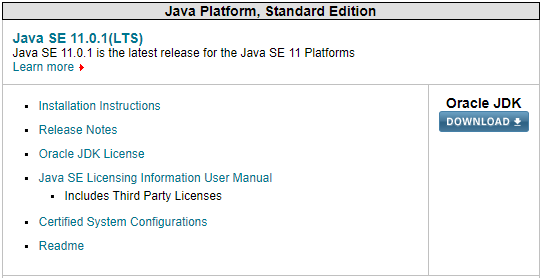
\includegraphics[scale=1.0]{image3/OracleJDK}
    \end{center}
    \caption{Oracle JDK}
    \label{refhinh1}
    \end{figure}
\end{center}
    \item nhấn chọn Accept License Agreement và sau đó chọn phiên bản phù hợp với hệ điều hành mà bạn đang sử dụng
\begin{center}
    \begin{figure}[htp]
    \begin{center}
     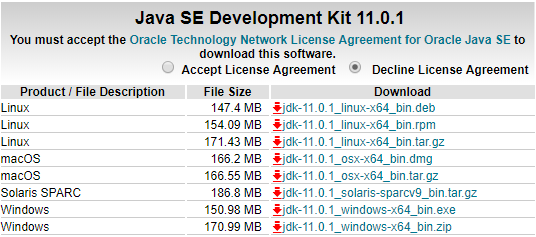
\includegraphics[scale=1.0]{image3/JDK}
    \end{center}
    \caption{Chọn Phiên bản JDK}
    \label{refhinh1}
    \end{figure}
\end{center}
\newpage
    \item Kết quả download được:
\begin{center}
    \begin{figure}[htp]
    \begin{center}
     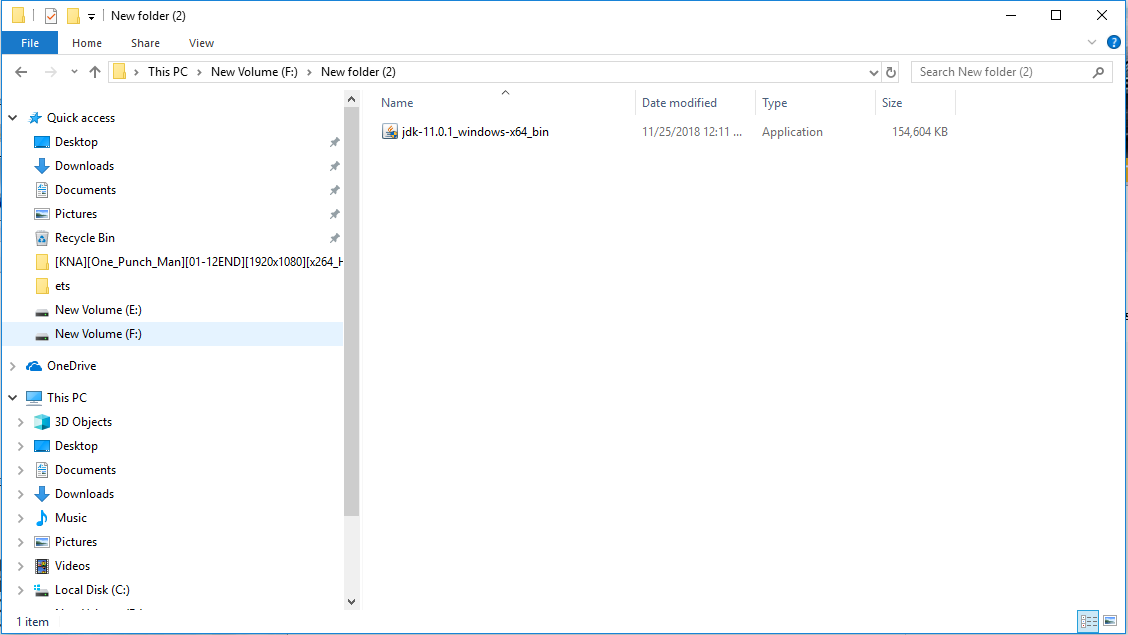
\includegraphics[scale=0.5]{image3/downloadjdk}
    \end{center}
    \caption{File JDK tải về}
    \label{refhinh1}
    \end{figure}
\end{center}
    \item chạy file vừa download về, nhấn next để tiếp tục.
\newpage
\begin{center}
    \begin{figure}[htp]
    \begin{center}
     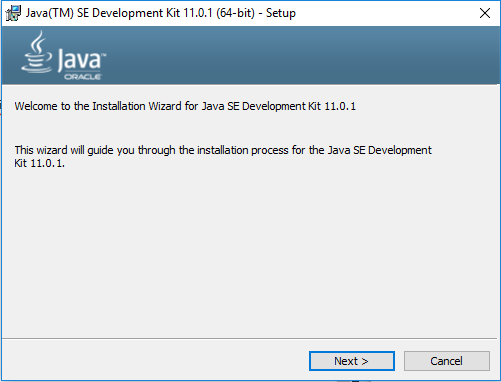
\includegraphics[scale=1.0]{image3/jdksetup}
    \end{center}
    \caption{Chạy File JDK tải về}
    \label{refhinh1}
    \end{figure}
\end{center}
    \item Nhập vào thư mục mà JDK sẽ được cài đặt ra, ở đây tôi đặt là: \textsf{C:Program File/Java/jdk-11.0.1/}
\newpage
\begin{center}
    \begin{figure}[htp]
    \begin{center}
     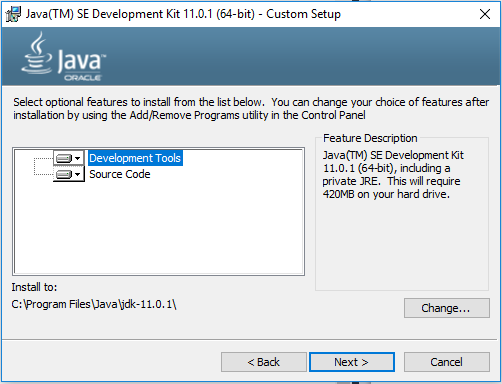
\includegraphics[scale=1.0]{image3/javatm}
    \end{center}
    \caption{Cài đặt đường dẫn file JDK tải về}
    \label{refhinh1}
    \end{figure}
\end{center}
    \item Nhấn next để tiếp tục, sau khi cài đặt xong nhấn close.
    \item Nhấn phải chuột vào Computer, chọn Properties. Sau đó nhấn Advance System Settings. Chon tiếp Advanced. Chọn Environment variables.
\newpage
\begin{center}
    \begin{figure}[htp]
    \begin{center}
     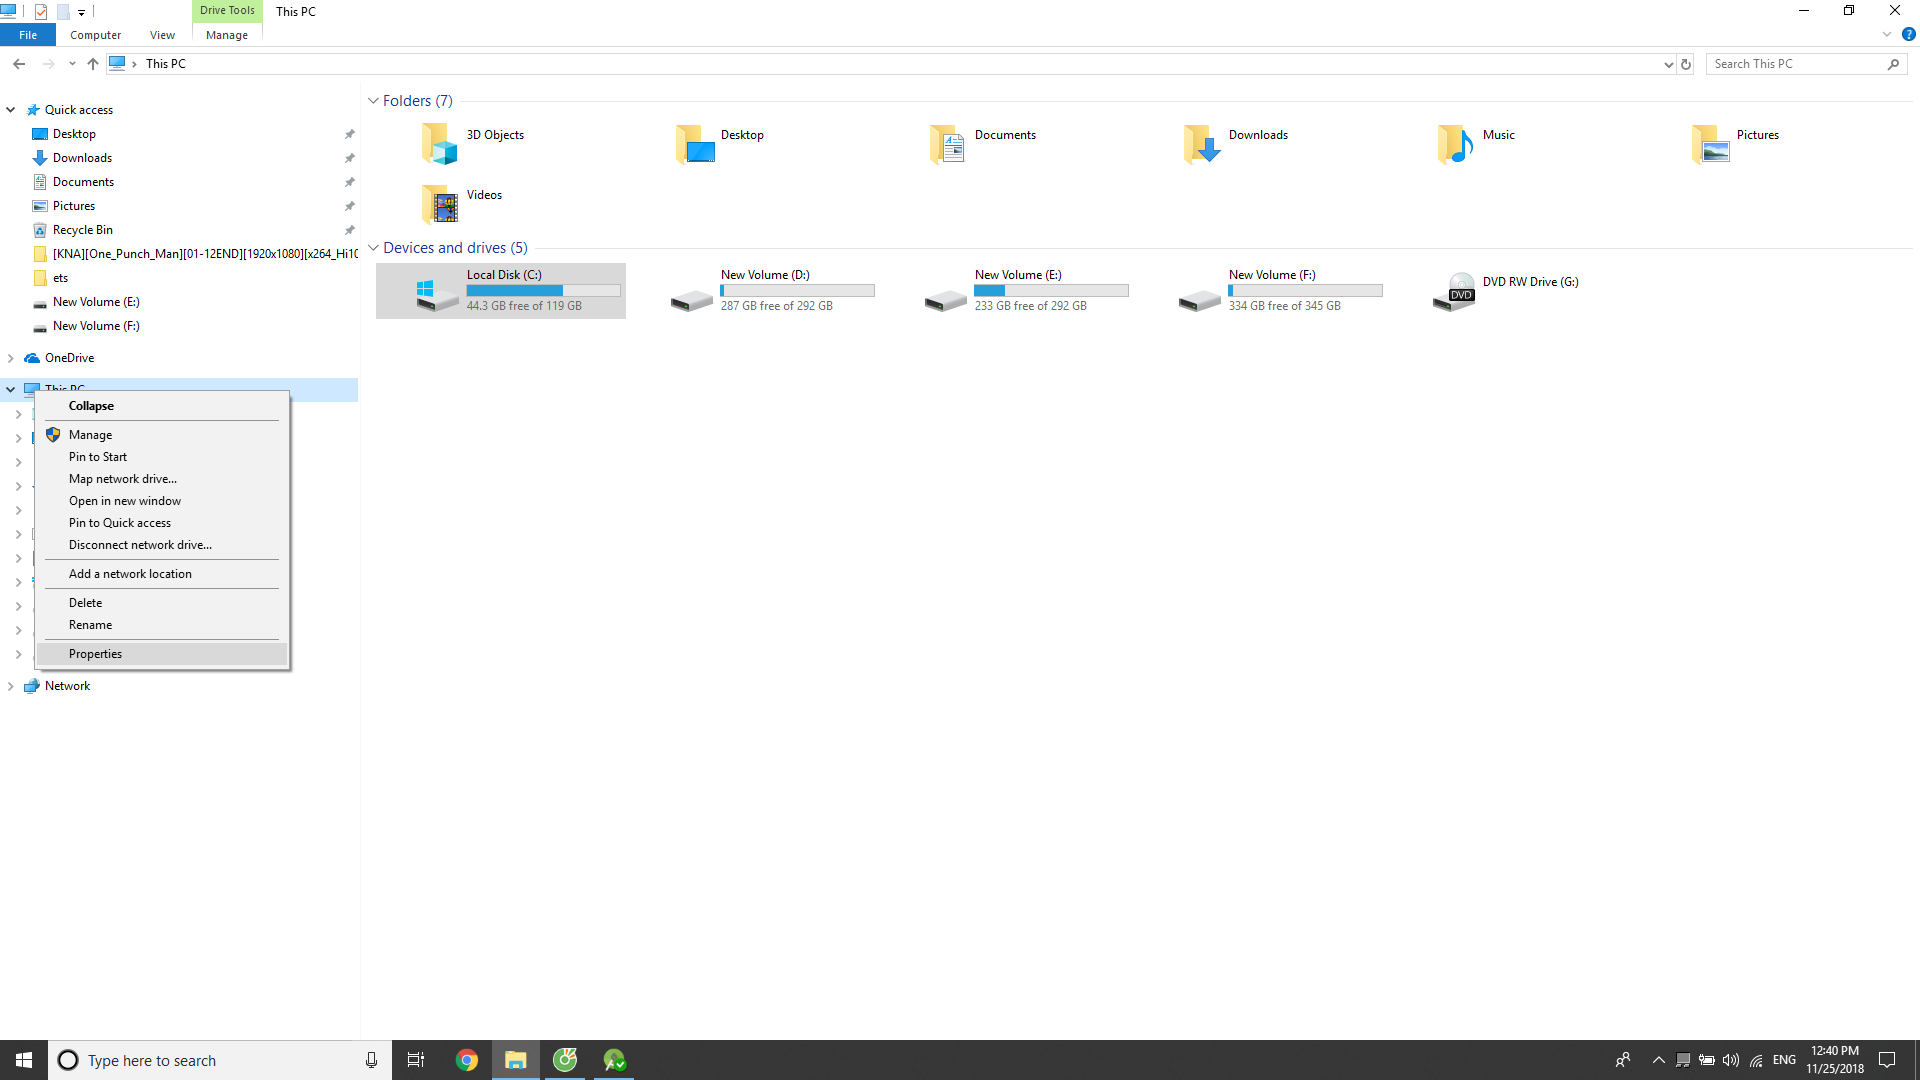
\includegraphics[scale=0.25]{image3/pc}
    \end{center}
    \caption{Chọn Properties.}
    \label{refhinh1}
    \end{figure}
\end{center}
\begin{center}
    \begin{figure}[htp]
    \begin{center}
     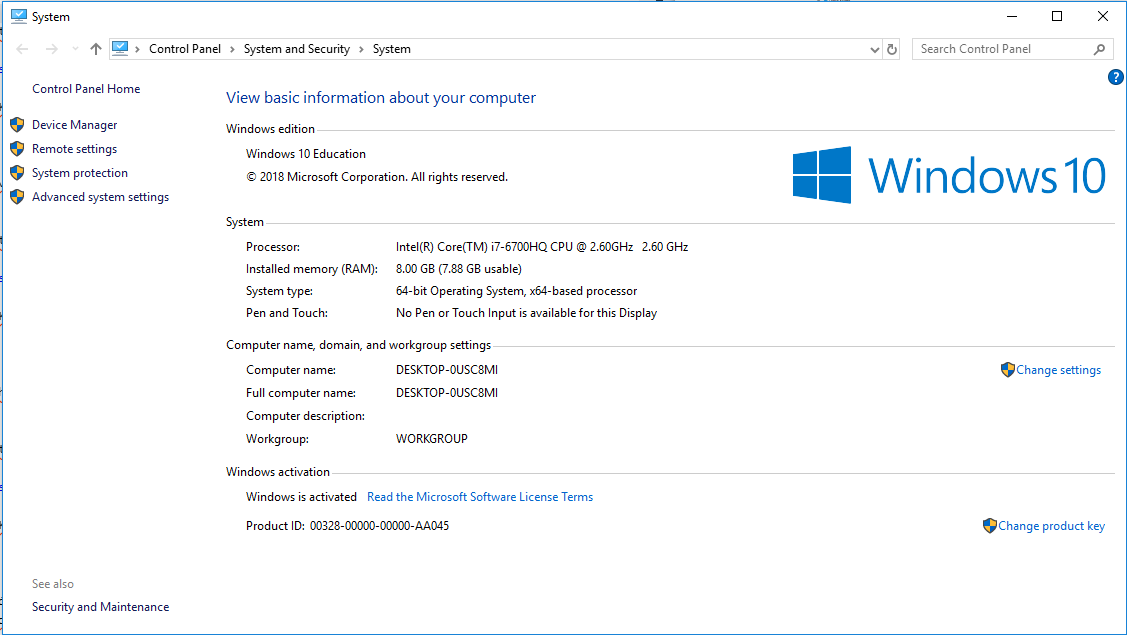
\includegraphics[scale=0.4]{image3/advanced}
    \end{center}
    \caption{Chọn Advanced System Settings.}
    \label{refhinh1}
    \end{figure}
\end{center}
\begin{center}
    \begin{figure}[htp]
    \begin{center}
     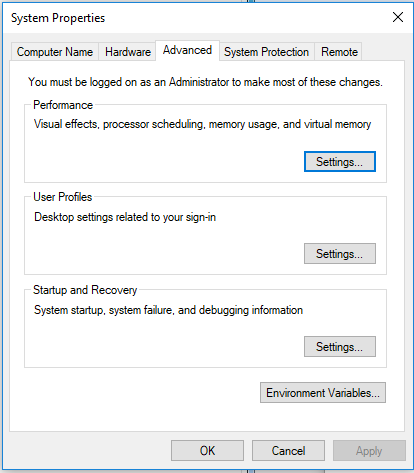
\includegraphics[scale=0.5]{image3/adv}
    \end{center}
    \caption{Chọn Advanced.}
    \label{refhinh1}
    \end{figure}
\end{center}
\newpage
    \item Nhấn New để tạo mới một biến môi trường có tên "JAVA\_HOME".
\begin{center}
    \begin{figure}[htp]
    \begin{center}
     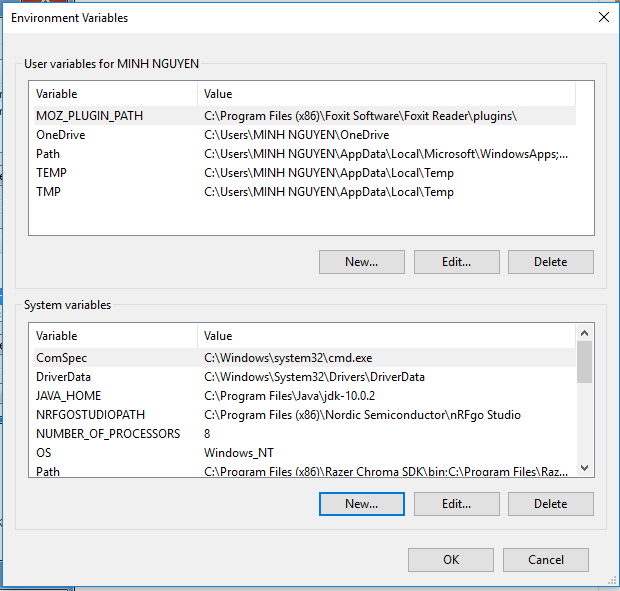
\includegraphics[scale=0.5]{image3/newjava}
    \end{center}
    \caption{Tạo một biến môi trường có tên "JAVA\_HOME".}
    \label{refhinh1}
    \end{figure}
\end{center}
\newpage
    \item Nhập vào đường dẫn tới thư mục JDK.\\
    Variable name: JAVA\_HOME\\
    Variable value: \textsf{C:/Program Files/Java/jdk-11.0.1}
\begin{center}
    \begin{figure}[htp]
    \begin{center}
     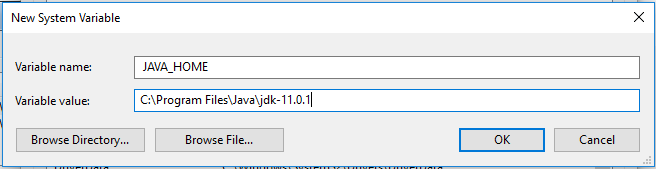
\includegraphics[scale=0.5]{image3/javahome}
    \end{center}
    \caption{Nhập Variable name và Variable value.}
    \label{refhinh1}
    \end{figure}
\end{center}
    \item Tiếp theo sửa đổi biến môi trường path\\
    Nhấn vào Edit, sau đó nhấn vào Edit text. Thêm vào phía trước giá trị của biến môi trường path:\textsf{\%JAVA\_HOME\%/bin;}
\begin{center}
    \begin{figure}[htp]
    \begin{center}
     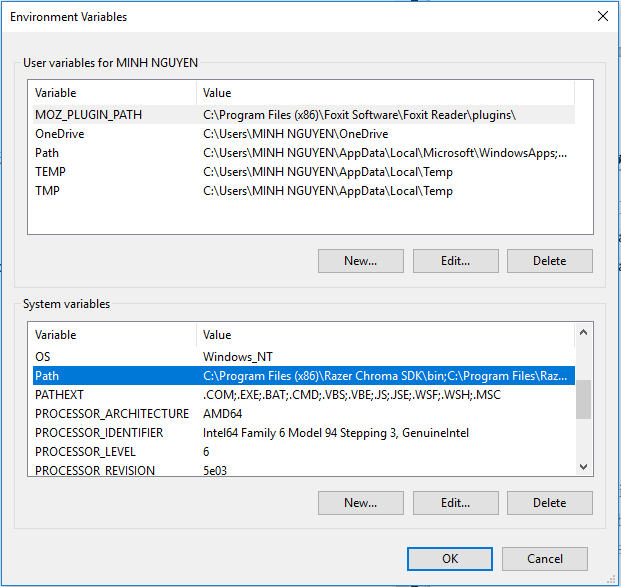
\includegraphics[scale=0.5]{image3/edit}
    \end{center}
    \caption{Nhấn vào Edit.}
    \label{refhinh1}
    \end{figure}
\end{center}
\newpage
\begin{center}
    \begin{figure}[htp]
    \begin{center}
     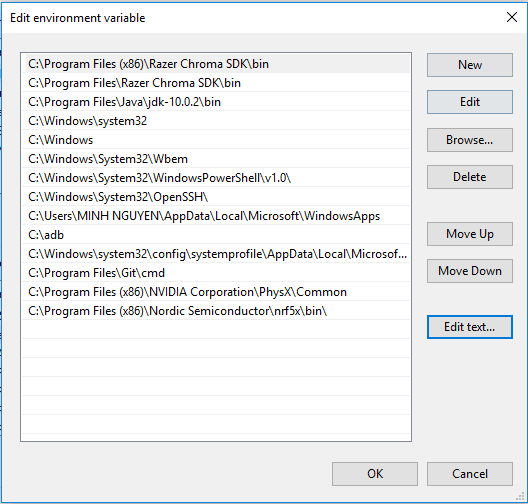
\includegraphics[scale=0.5]{image3/edittext}
    \end{center}
    \caption{Nhấn vào Edit text.}
    \label{refhinh1}
    \end{figure}
\end{center}
\begin{center}
    \begin{figure}[htp]
    \begin{center}
     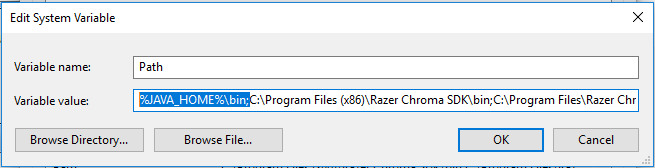
\includegraphics[scale=0.5]{image3/javaedit}
    \end{center}
    \caption{Hoàn tất thêm vào "\%JAVA\_HOME\%/bin".}
    \label{refhinh1}
    \end{figure}
\end{center}
 \end{enumerate}
 \subsection{Cài đặt Android Studio}
 Có nhiều công cụ để phát triển Android nhưng đến nay công cụ chính thức và mạnh mẽ nhất là Android Studio. Đây là IDE (Môi trường phát triển tích hợp) chính thức cho nền tảng Android, được phát triển bởi Google và được sử dụng để tạo phần lớn các ứng dụng mà bạn có thể sử dụng hàng ngày.
 
 Android Studio lần đầu tiên được công bố tại hội nghị Google I/O vào năm 2013 và được phát hành cho công chúng vào năm 2014 sau nhiều phiên bản beta khác nhau. Trước khi được phát hành, các nhà phát triển Android thường sử dụng các công cụ như Eclipse IDE, một IDE Java chung cũng hỗ trợ nhiều ngôn ngữ lập trình khác.
 
 Android Studio khiến việc tạo ứng dụng trở nên dễ dàng hơn đáng kể so với phần mềm không chuyên dụng. Đối với người mới bắt đầu, có rất nhiều thứ để học và nhiều thông tin có sẵn, thậm chí thông qua các kênh chính thức nhưng chúng có thể đã lỗi thời hoặc quá nhiều thông tin khiến họ cảm thấy choáng ngợp.
 
 Chức năng của Android Studio là cung cấp giao diện để tạo các ứng dụng và xử lý phần lớn các công cụ quản lý file phức tạp đằng sau hậu trường. Ngôn ngữ lập trình được sử dụng ở đây là Java và được cài đặt riêng trên thiết bị của bạn. Android Studio rất đơn giản, bạn chỉ cần viết, chỉnh sửa và lưu các dự án của mình và các file trong dự án đó. Đồng thời, Android Studio sẽ cấp quyền truy cập vào Android SDK.
 
 Hãy coi đây là đuôi cho code Java cho phép nó chạy trơn tru trên các thiết bị Android và tận dụng lợi thế của phần cứng gốc. Bạn cần sử dụng ngôn ngữ lập trình Java để viết các chương trình, Android SDK có nhiệm vụ kết nối các phần này lại với nhau. Cùng lúc đó Android Studio kích hoạt để chạy code, thông qua trình giả lập hoặc qua một phần cứng kết nối với thiết bị. Sau đó, bạn cũng có thể “gỡ rối” chương trình khi nó chạy và nhận phản hồi giải thích sự cố, v.v… để bạn có thể nhanh chóng giải quyết vấn đề.
 
 Google đã nỗ lực rất nhiều để làm cho Android Studio trở nên mạnh mẽ và hữu ích nhất có thể. Nó cung cấp những gợi ý trực tiếp trong khi viết code và thường đề xuất những thay đổi cần thiết để sửa lỗi hoặc làm code hiệu quả hơn. Ví dụ, nếu không sử dụng biến, biến đó sẽ được tô đậm bằng màu xám. Và khi bắt đầu gõ một dòng code, Android Studio sẽ cung cấp danh sách gợi ý tự hoàn thành để giúp bạn hoàn thiện dòng code đó. Chức năng này rất hữu ích khi bạn không nhớ được chính xác cú pháp hoặc để tiết kiệm thời gian\cite{tl3}.
 
 Hướng dẫn cài đặt android stuido.
 \begin{enumerate}
     \item Vào trang web \url{https://developer.android.com/studio/} để download android studio.
\newpage
\begin{center}
    \begin{figure}[htp]
    \begin{center}
     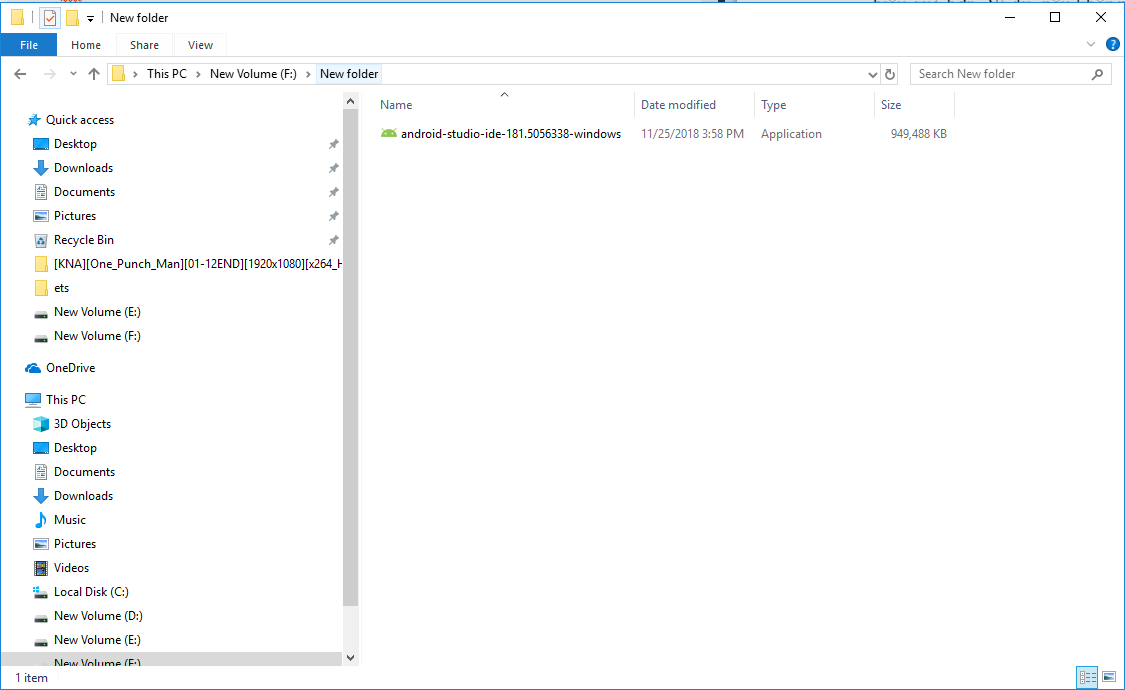
\includegraphics[scale=0.45]{image3/androidstudio}
    \end{center}
    \caption{File android studio.}
    \label{refhinh1}
    \end{figure}
\end{center}
    \item Chạy file android studio tải về 
\begin{center}
    \begin{figure}[htp]
    \begin{center}
     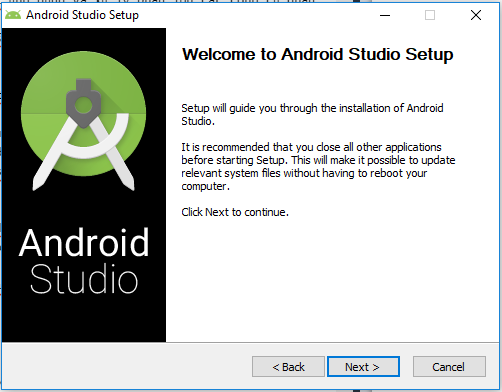
\includegraphics[scale=0.6]{image3/caidat1}
    \end{center}
    \caption{Nhấn Next để cài đặt.}
    \label{refhinh1}
    \end{figure}
\end{center}
\newpage
\begin{center}
    \begin{figure}[htp]
    \begin{center}
     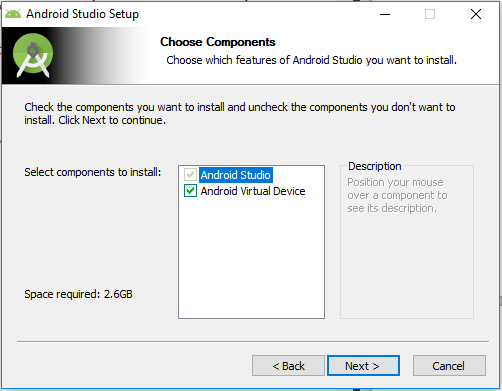
\includegraphics[scale=0.6]{image3/caidat2}
    \end{center}
    \caption{Nhấn Next để cài đặt.}
    \label{refhinh1}
    \end{figure}
\end{center}

\begin{center}
    \begin{figure}[htp]
    \begin{center}
     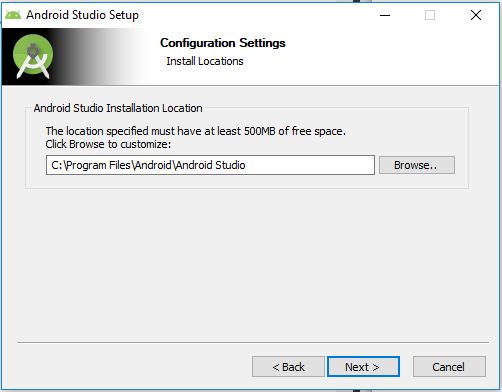
\includegraphics[scale=0.6]{image3/caidat3}
    \end{center}
    \caption{Chọn ví trí lưu, nhấn Next để cài đặt.}
    \label{refhinh1}
    \end{figure}
\end{center}
\newpage
\begin{center}
    \begin{figure}[htp]
    \begin{center}
     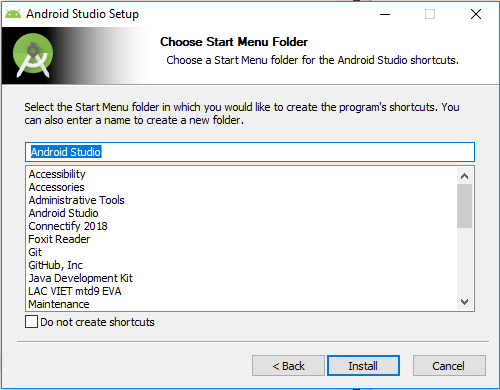
\includegraphics[scale=0.6]{image3/caidat4}
    \end{center}
    \caption{Nhấn Install để cài đặt.}
    \label{refhinh1}
    \end{figure}
\end{center}

\begin{center}
    \begin{figure}[htp]
    \begin{center}
     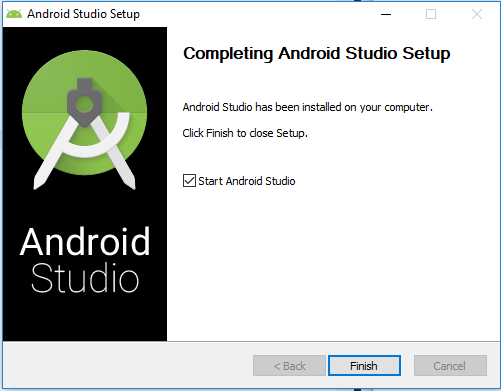
\includegraphics[scale=0.6]{image3/caidat5}
    \end{center}
    \caption{Nhấn Finish để cài đặt.}
    \label{refhinh1}
    \end{figure}
\end{center}
 \end{enumerate}
 
\newpage
\subsection{Cài đặt hệ điều hành Android Things}
Để cài hệ điều hành Android Things, cần thực hiện theo 3 bước sau.\\
Bước 1: Tạo Image Boot cho hệ điều hành Android Things.
\begin{enumerate}
\item Vào trang \url{https://partner.android.com/things/console/}, đăng nhập với tài khoản của Google. Nên sử dụng trình duyệt \href{https://www.google.com/chrome/}{Google Chrome} để tránh trường hơp không vào được trang
\begin{center}
\begin{figure}[htp]
\begin{center}
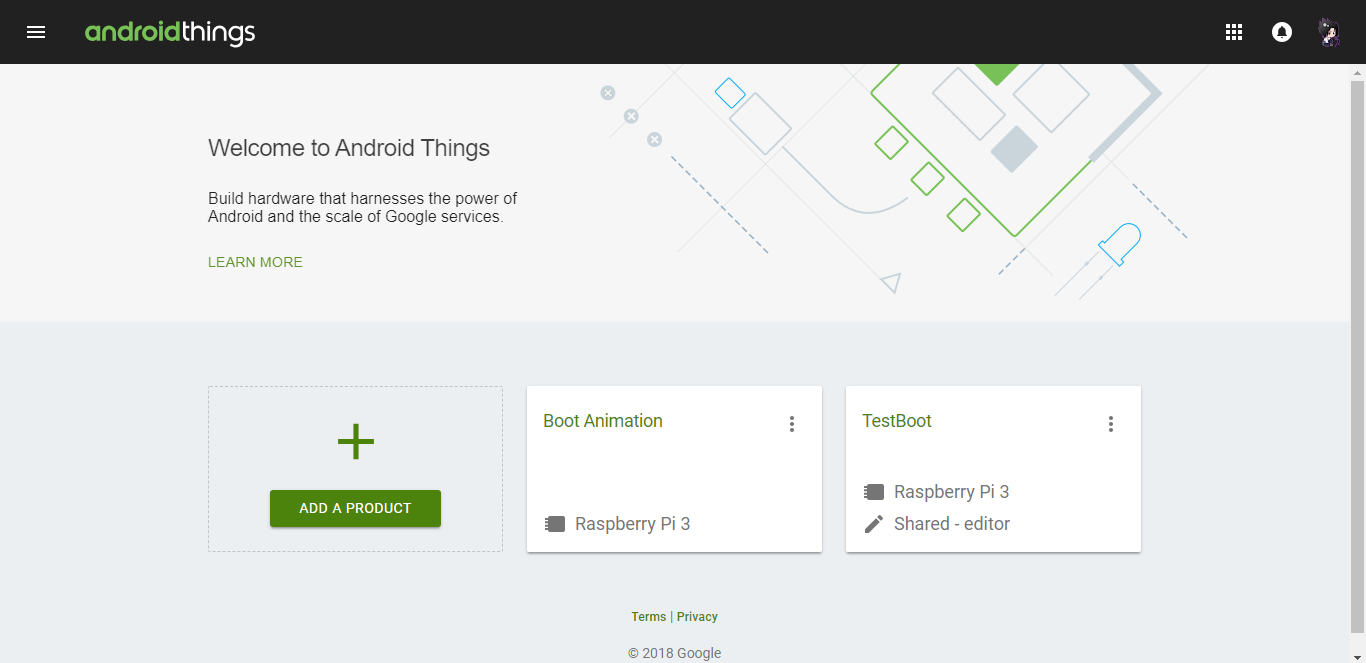
\includegraphics[scale=0.4]{image3/sat1.png}
\end{center}
\caption{Màn hình giao diện - tạo Image Boot.}
\label{refhinh1}
\end{figure}
\end{center}
\item Nhấn vào "ADD A PRODUCT" hoặc biểu tượng dấu cộng "+".
\begin{center}
\begin{figure}[htp]
\begin{center}
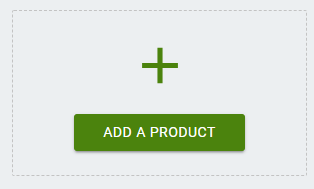
\includegraphics[scale=1]{image3/sat2.png}
\end{center}
\caption{Nhấn + để tạo PRODUCT mới.}
\label{refhinh1}
\end{figure}
\end{center}
\item Bảng "Create new product" hiện lên. Điền thông tin vào các trường: 
\begin{center}
\begin{figure}[htp]
\begin{center}
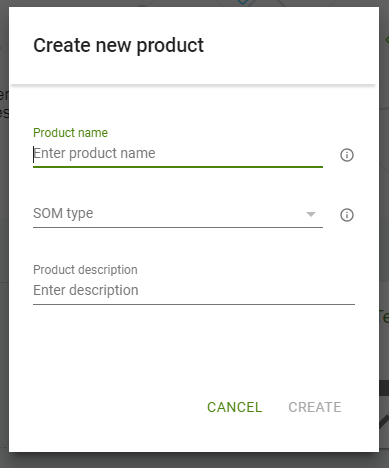
\includegraphics[scale=0.8]{image3/sat3.png}
\end{center}
\caption{Thêm thông tin PRODUCT vào bảng.}
\label{refhinh1}
\end{figure}
\end{center}
\begin{itemize}
\item "Product name" - là tên sản phẩm mà mình sẽ làm việc, yêu cầu có ít nhất một ký tự chữ, ví dụ "Starter".
\item "SOM type" - là mạch phần cứng được sử dụng, ở đây dùng Rpi3 nên chọn "Raspberry Pi 3".
\item "Product description" là mô tả về sản phẩm, trường này không bắt buộc phải điền 
\end{itemize}
\item Sau khi điền xong, nhấn "Create" để tạo sản phẩm.
\begin{center}
\begin{figure}[htp]
\begin{center}
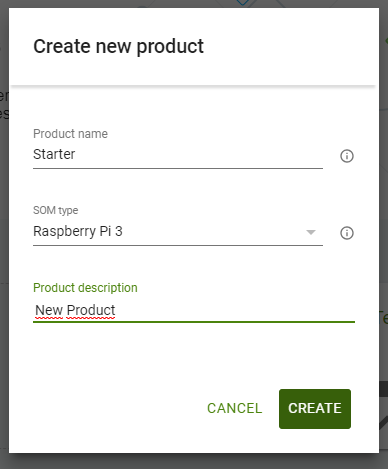
\includegraphics[scale=0.6]{image3/sat4.png}
\end{center}
\caption{Nhấn CREATE để tạo sản phẩm.}
\label{refhinh1}
\end{figure}
\end{center}
\newpage
\item Sau khi tạo xong, màn hình sẽ hiện ra kết quả khi tạo thành công, ấn vô ô ("ei3ri4" - theo ví dụ) ở phần "Models".
\begin{center}
\begin{figure}[htp]
\begin{center}
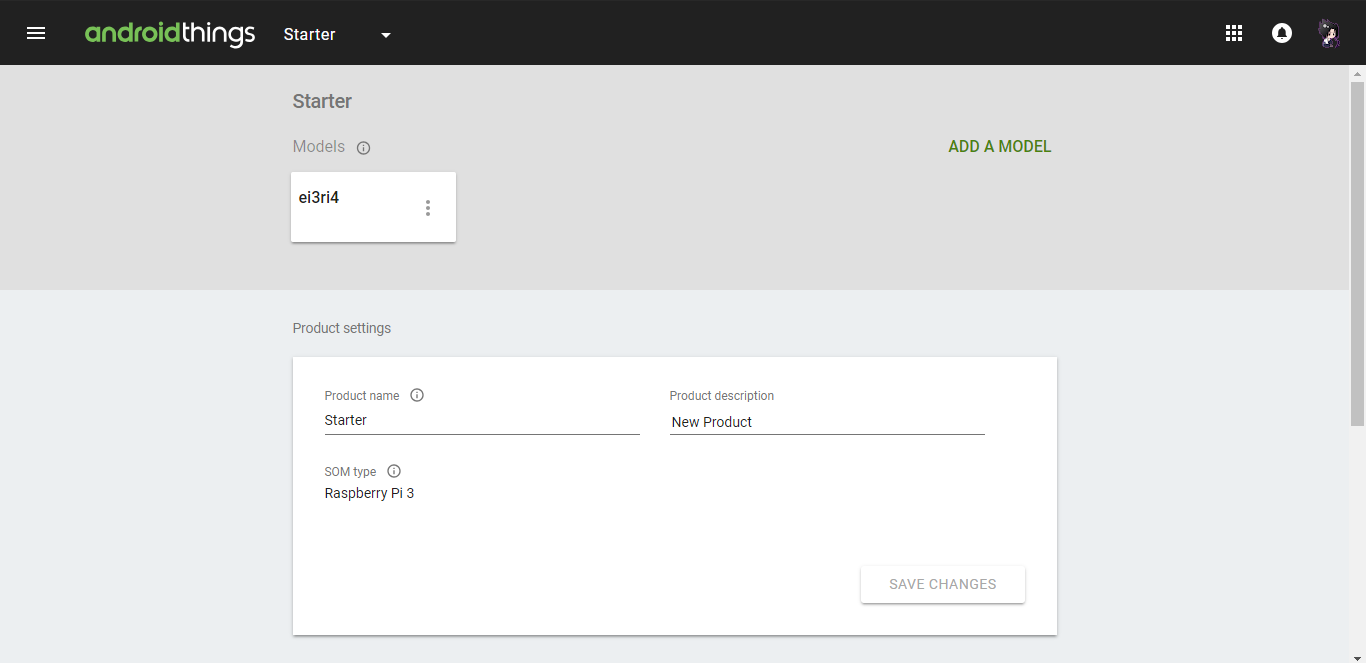
\includegraphics[scale=0.4]{image3/sat5.png}
\end{center}
\caption{Tạo thành công sản phẩm.}
\label{refhinh1}
\end{figure}
\end{center}
\item Tại tab "BUILD", ấn vào nút "NEW" ở gần bên phải giữa màn hình để tạo mới một Image Boot.
\begin{center}
\begin{figure}[!htp]
\begin{center}
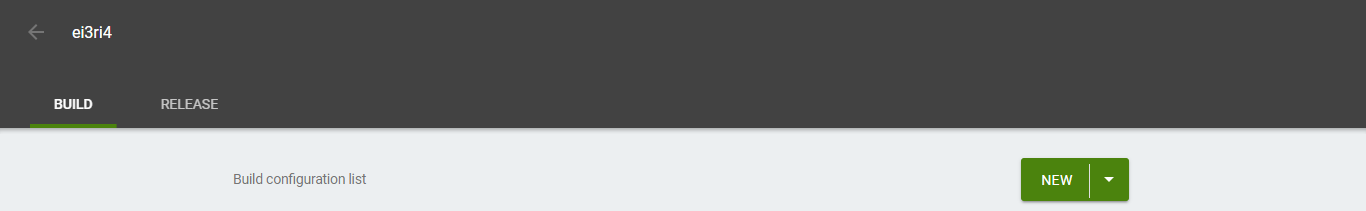
\includegraphics[scale=0.4]{image3/sat6.png}
\end{center}
\caption{Ấn NEW để tạo mới Image Boot.}
\label{refhinh1}
\end{figure}
\end{center}
\newpage
\item Tại khung xổ xuống, chọn "Start from scratch".
\begin{center}
\begin{figure}[htp]
\begin{center}
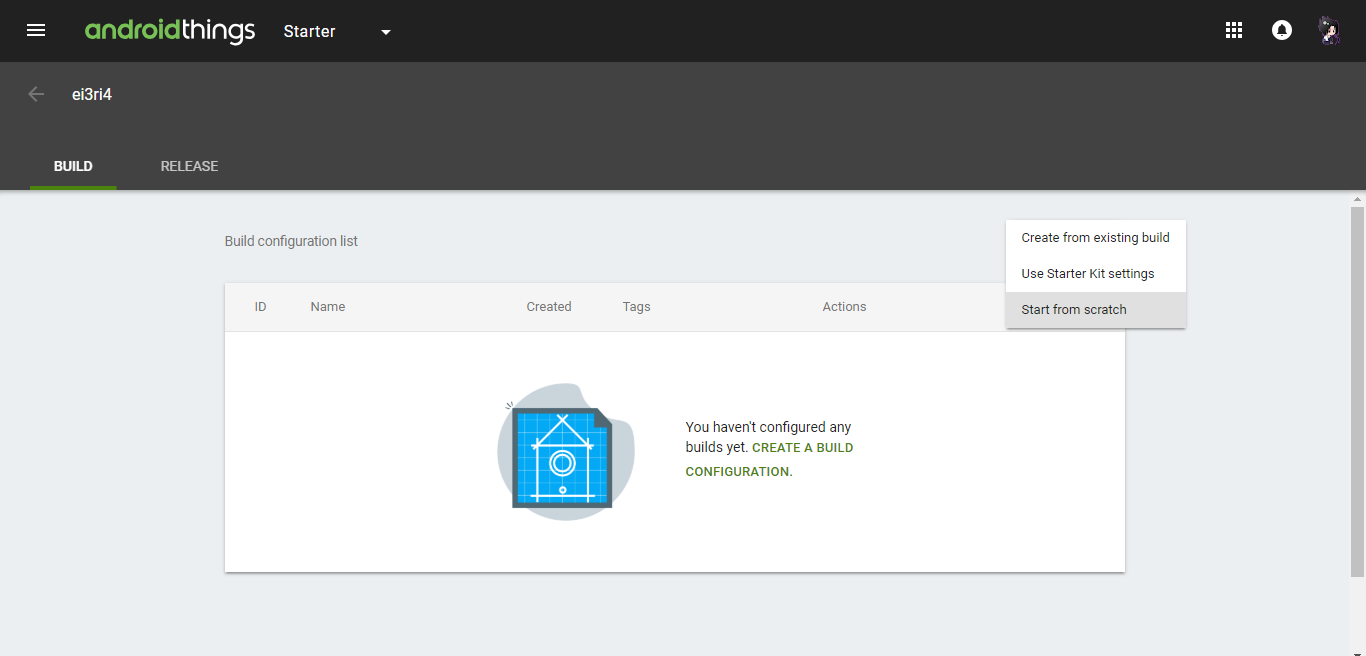
\includegraphics[scale=0.38]{image3/sat7.png}
\end{center}
\caption{Chọn Start from scratch.}
\label{refhinh1}
\end{figure}
\end{center}
\item Tại trường "1", nhập tên Image Boot muốn tạo, ví dụ "New Build". Sau đó ấn "NEXT".
\begin{center}
\begin{figure}[htp]
\begin{center}
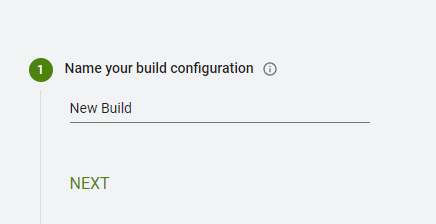
\includegraphics[scale=0.65]{image3/sat8.png}
\end{center}
\caption{Nhập tên Image Boot.}
\label{refhinh1}
\end{figure}
\end{center}
\item Tại trường "2", chọn phiên bản Android Things mới nhất, thường có chữ "(latest)" ở cột "OS version". Sau đó ấn "NEXT".
\begin{center}
\begin{figure}[htp]
\begin{center}
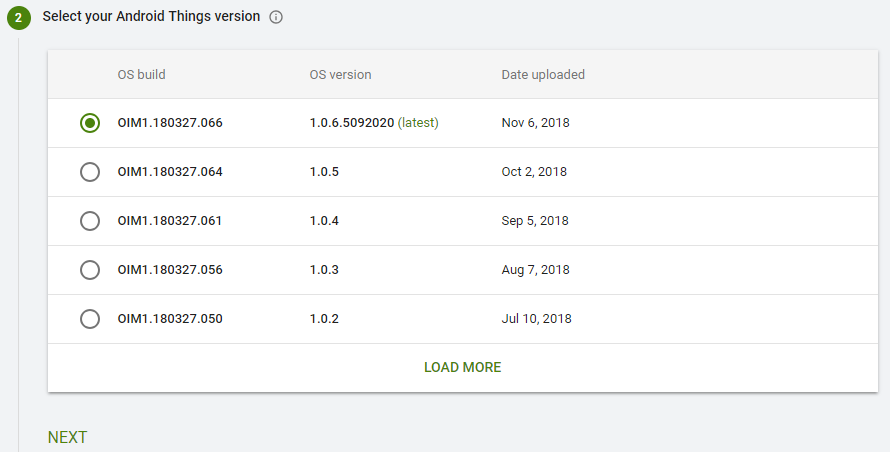
\includegraphics[scale=0.6]{image3/sat9.png}
\end{center}
\caption{Chọn phiên bản Android Things mới nhất.}
\label{refhinh1}
\end{figure}
\end{center}
\item Trường "3" là nơi để upload ứng dụng được chạy tự động đầu tiên sau khi hệ điều hành được khởi động. Nếu muốn thiết lập cho ứng dụng tự khởi chạy thì ấn chọn "SELECT APPS". Nhưng vẫn khuyên không nên chọn và ấn "NEXT".
\begin{center}
\begin{figure}[htp]
\begin{center}
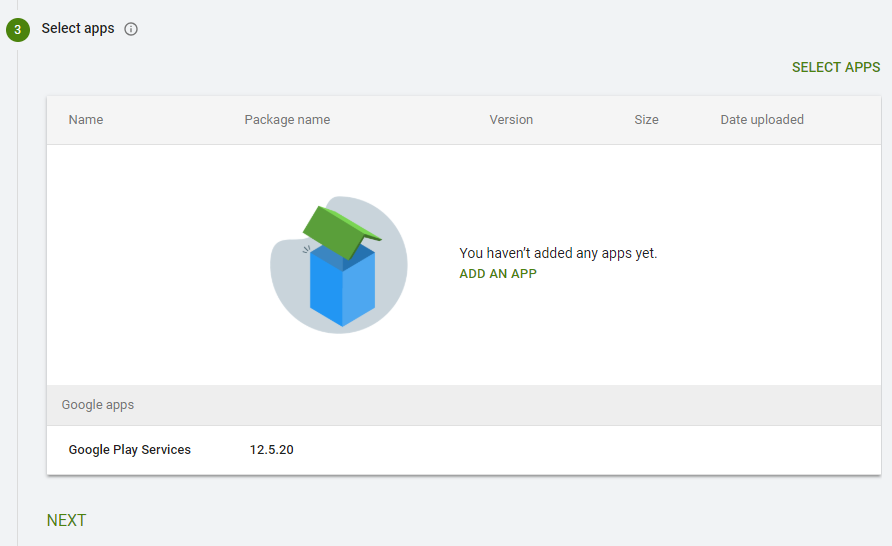
\includegraphics[scale=0.5]{image3/sat10.png}
\end{center}
\caption{Chọn NEXT tại bước này.}
\label{refhinh1}
\end{figure}
\end{center}
\item \label{truong4} Trường "4" sẽ là nơi để cài đặt hình ảnh load đầu tiên khi hệ điều hành được khởi động. Có thể thay đổi hình ảnh này, điều này sẽ được hướng dẫn thêm ở \hyperref[bootanimation]{mục \ref*{bootanimation}}. Sau đó ấn "NEXT".
\begin{center}
\begin{figure}[htp]
\begin{center}
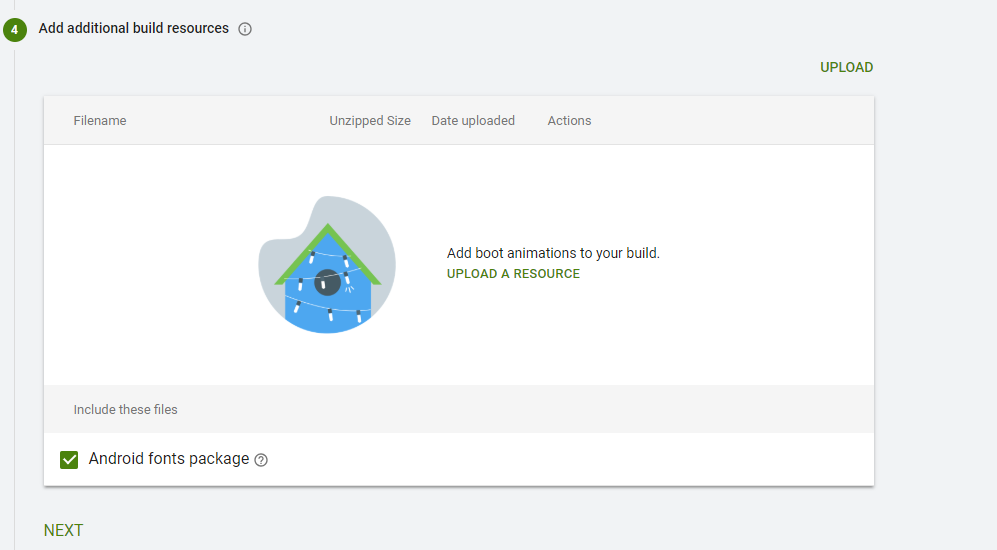
\includegraphics[scale=0.45]{image3/sat11.png}
\end{center}
\caption{Chọn NEXT tại bước này -  \hyperref[bootanimation]{Xem thêm \ref*{bootanimation}}.}
\label{refhinh1}
\end{figure}
\end{center}
\item \label{truong5} Trường "5" là phần chỉnh sửa thông tin về chân cắm của phần cứng. KHÔNG NÊN CAN THIỆP VÀO PHẦN NÀY, chỉ nên can thiệp nếu đã đủ khả năng làm việc với mạch. Sau đó ấn "NEXT".
\begin{center}
\begin{figure}[htp]
\begin{center}
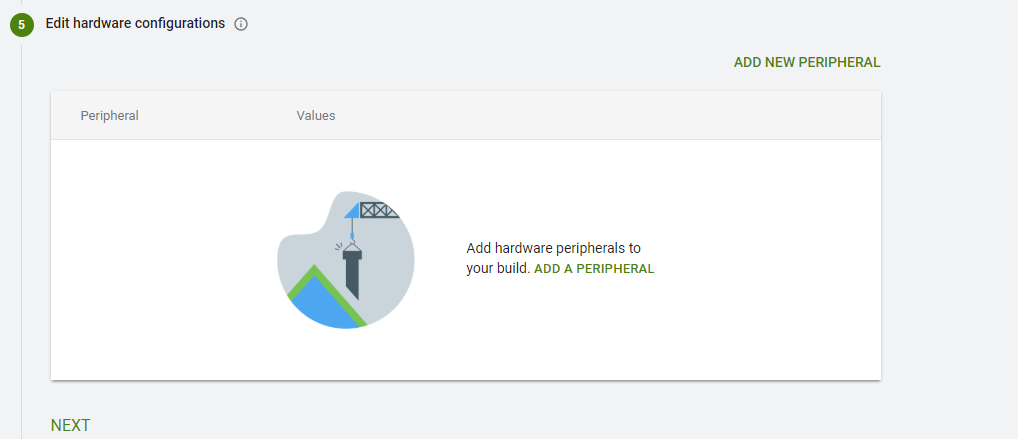
\includegraphics[scale=0.5]{image3/sat12.png}
\end{center}
\caption{Chọn NEXT tại bước này.}
\label{refhinh1}
\end{figure}
\end{center}
\item Tại trường "6" sẽ thống kê lại những thiết lập đã chọn. Ấn "CREATE BUILD" để tạo Image Boot.
\begin{center}
\begin{figure}[htp]
\begin{center}
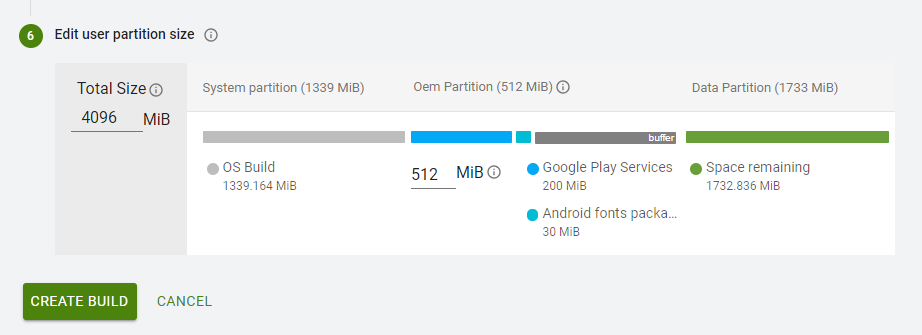
\includegraphics[scale=0.6]{image3/sat13.png}
\end{center}
\caption{Thông tin về bản Image Boot.}
\label{refhinh1}
\end{figure}
\end{center}
\newpage
\item Vậy là đã tạo xong một bản Image Boot rồi.
\begin{center}
\begin{figure}[htp]
\begin{center}
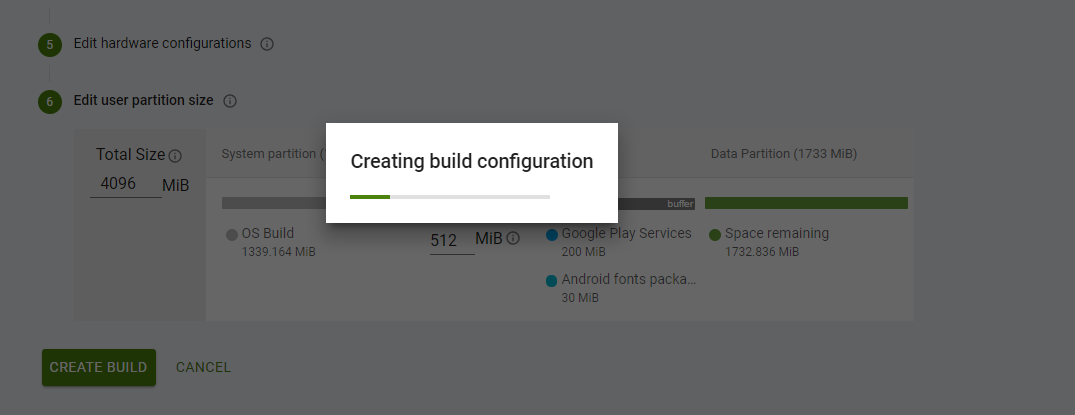
\includegraphics[scale=0.45]{image3/sat14.png}
\end{center}
\caption{Ấn CREATE BUILD để tạo.}
\label{refhinh1}
\end{figure}
\end{center}
\item Để tải bản Image Boot, tại cột "Actions", ấn vô "Download".
\begin{center}
\begin{figure}[htp]
\begin{center}
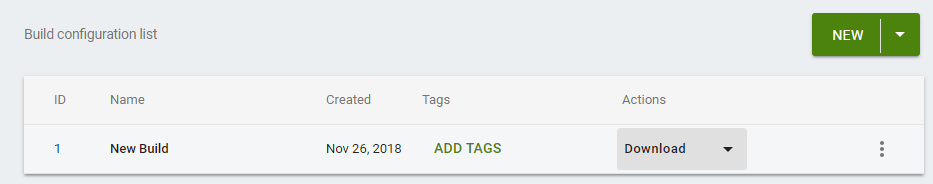
\includegraphics[scale=0.52]{image3/sat17.png}
\end{center}
\caption{Ấn Download tại bản Image Boot muốn tải.}
\label{refhinh1}
\end{figure}
\end{center}
\newpage
\item Tiếp tục ấn vô "Development" để thực hiện quá trình tải.
\begin{center}
\begin{figure}[htp]
\begin{center}
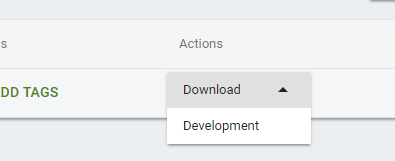
\includegraphics[scale=0.7]{image3/sat18.png}
\end{center}
\caption{Chọn Development.}
\label{refhinh1}
\end{figure}
\end{center}
\item Đợi từ 5 đến 10 phút là tải xong (tùy thuộc vào tốc độ mạng).
\begin{center}
\begin{figure}[htp]
\begin{center}
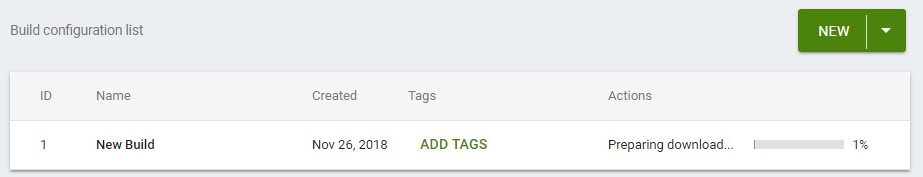
\includegraphics[scale=0.6]{image3/sat19.png}
\end{center}
\caption{Chờ để tải xuống.}
\label{refhinh1}
\end{figure}
\end{center}
\item File Image Boot đã tải xong, dung lượng tầm khoảng 300 - 350 (MB), định dạng file là ".zip".
\begin{center}
\begin{figure}[htp]
\begin{center}
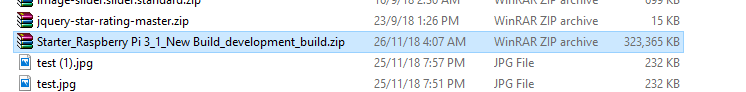
\includegraphics[scale=0.75]{image3/sat20.png}
\end{center}
\caption{Đã tải thành công.}
\label{refhinh1}
\end{figure}
\end{center}
\end{enumerate}
Bước 2: Cài đặt hệ điều hành lên thẻ nhớ (dung lượng từ 8GB trở lên).\\
\hspace*{0.25cm}Cách 1: Sử dụng phần mềm \href{https://www.sdcard.org/downloads/formatter_4/}{SD Card Formatter}, \href{https://sourceforge.net/projects/win32diskimager/}{Win32 Disk Image}.
\newpage
\begin{enumerate}
\item Cắm thẻ nhớ MicroSD vào đầu đọc thẻ, sau đó cắm vào máy tính. Sẽ hiện ra thông báo yêu cầu định dạng lại thẻ nhớ, nhấn "Cancel".
\begin{center}
\begin{figure}[htp]
\begin{center}
 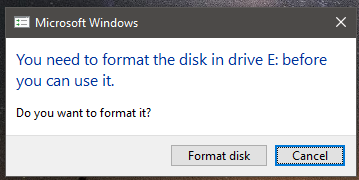
\includegraphics[scale=0.8]{image3/buoc2cach1s1.png}
\end{center}
\caption{Nhấn Cancel sau khi cắm thẻ nhớ vô máy.}
\label{refhinh1}
\end{figure}
\end{center}
\item Chạy phần mềm SD Card Formatter để định dạng thẻ nhớ. Lưu ý, phải chọn đứng ổ đĩa của thẻ nhớ để tránh trường hợp định dạng nhầm ổ cứng máy tính. Ấn "Refresh" để tự động tìm thẻ nhớ đã được kết nối.
\begin{center}
\begin{figure}[htp]
\begin{center}
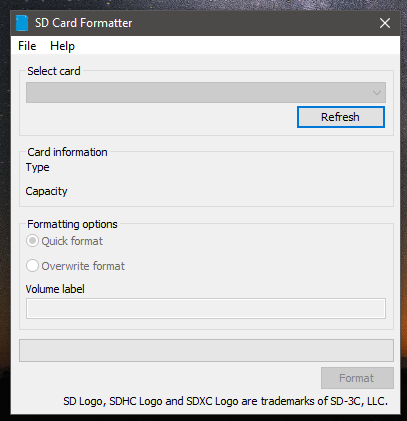
\includegraphics[scale=0.75]{image3/buoc2cach1s2.png}
\end{center}
\caption{Nhấn Refresh để tự động tìm thẻ nhớ.}
\label{sdcardformat}
\end{figure}
\end{center}
\item Sau khi tìm được, chọn thẻ nhớ dùng để cài hệ điều hành. Nhấn "Format" để định dạng.
\begin{center}
\begin{figure}[htp]
\begin{center}
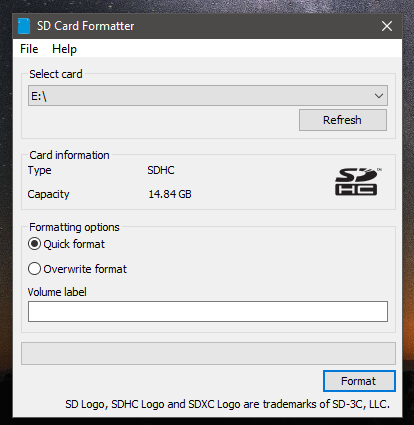
\includegraphics[scale=0.7]{image3/buoc2cach1s3.png}
\end{center}
\caption{Nhấn Format để định dạng.}
\label{refhinh1}
\end{figure}
\end{center}
\item Thông báo nhắc nhở sẽ hiện lên, nhấn "Yes" để thực hiện quá trình định dạng thẻ nhớ.
\begin{center}
\begin{figure}[htp]
\begin{center}
 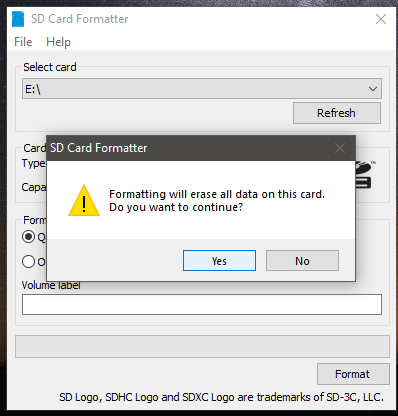
\includegraphics[scale=0.65]{image3/buoc2cach1s4.png}
\end{center}
\caption{Nhấn Yes.}
\label{refhinh1}
\end{figure}
\end{center}
\item Định dạng xong, phần mềm sẽ hiển thị như  \hyperref[finishformat]{hình \ref*{finishformat}}. Nhấn "OK" và thoát.
\begin{center}
\begin{figure}[htp]
\begin{center}
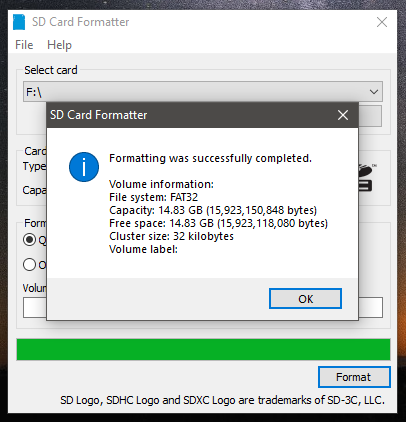
\includegraphics[scale=0.7]{image3/buoc2cach1s5.png}
\end{center}
\caption{Nhấn OK.}
\label{finishformat}
\end{figure}
\end{center}
\item Giải nén tập tin Image Boot vừa tải xong. Sau khi giải nén xong sẽ có một tập tin "iot\_rpi3.img".
\begin{center}
\begin{figure}[htp]
\begin{center}
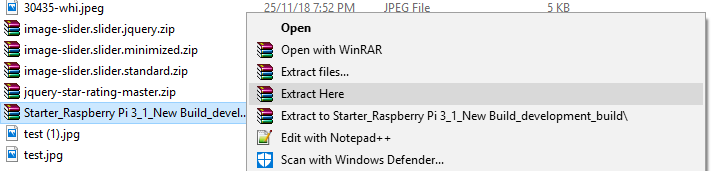
\includegraphics[scale=0.6]{image3/buoc2cach1s6.png}
\end{center}
\caption{Giải nén tập tin Image Boot vừa tải.}
\label{refhinh1}
\begin{center}
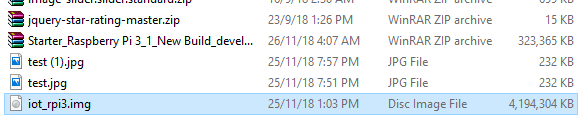
\includegraphics[scale=0.73]{image3/buoc2cach1s7.png}
\end{center}
\caption{Nhận được tập tin "iot\_rpi3.img".}
\label{refhinh1}
\end{figure}
\end{center}
\item Chạy phần mềm Win32 Disk Image để cài hệ điều hành lên thẻ nhớ.
\begin{center}
\begin{figure}[htp]
\begin{center}
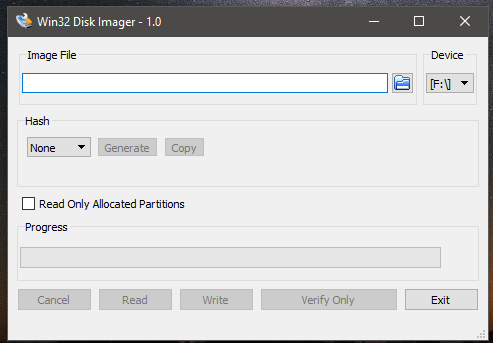
\includegraphics[scale=0.65]{image3/buoc2cach1s8.png}
\end{center}
\caption{Chạy phần mềm Win32 Disk Image.}
\label{refhinh1}
\end{figure}
\end{center}
\newpage
\item Chọn đường dẫn tới tập tin "iot\_rpi3.img" vừa được giải nén xong. Ví dụ: \textsf{C:/Download/}
\begin{center}
\begin{figure}[htp]
\begin{center}
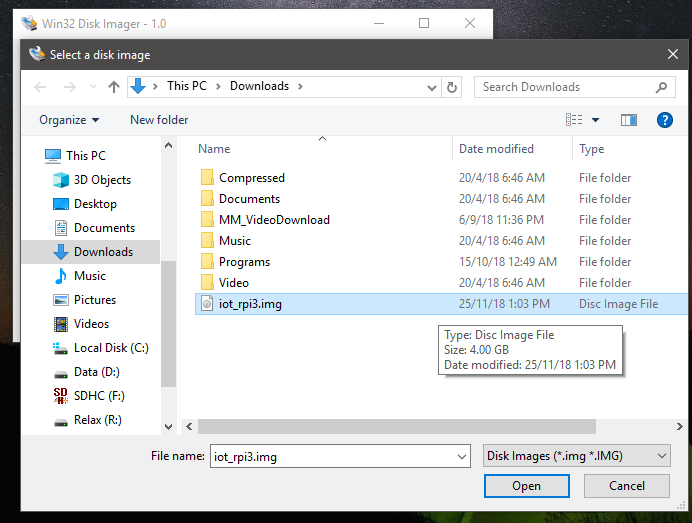
\includegraphics[scale=0.6]{image3/buoc2cach1s9.png}
\end{center}
\caption{Chọn đường dẫn tới tập tin Image Boot đã được giải nén.}
\label{refhinh1}
\end{figure}
\end{center}
\newpage
\item Chọn thẻ nhớ đã được định dạng.
\begin{center}
\begin{figure}[htp]
\begin{center}
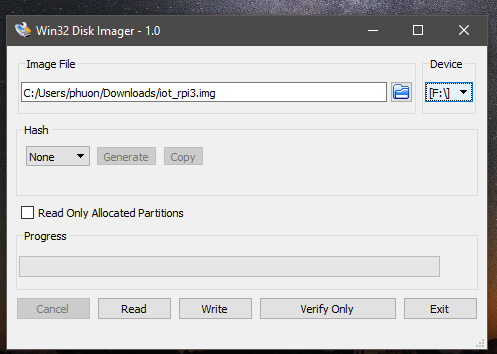
\includegraphics[scale=0.65]{image3/buoc2cach1s10.png}
\end{center}
\caption{Chọn thẻ nhớ.}
\label{refhinh1}
\end{figure}
\end{center}
\item Ấn "Write" để ghi hệ điều hành Android Things vào thẻ nhớ.
\begin{center}
\begin{figure}[htp]
\begin{center}
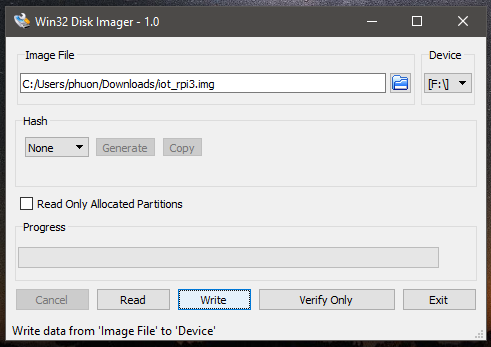
\includegraphics[scale=0.67]{image3/buoc2cach1s11.png}
\end{center}
\caption{Chọn thẻ nhớ.}
\label{refhinh1}
\end{figure}
\end{center}
\item Chương trình sẽ hiện ra tin nhắn cảnh báo, ấn "Yes" để tiếp tục quá trình.
\begin{center}
\begin{figure}[htp]
\begin{center}
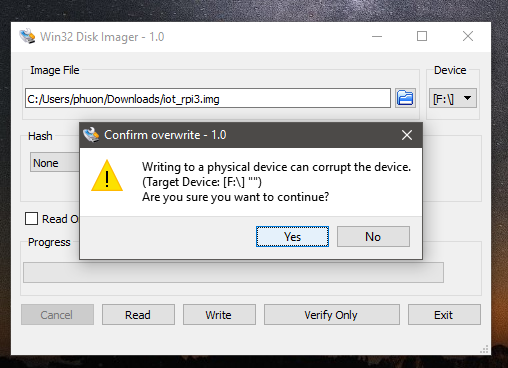
\includegraphics[scale=0.65]{image3/buoc2cach1s12.png}
\end{center}
\caption{Nhấn Yes để tiếp tục.}
\label{refhinh1}
\end{figure}
\end{center}
\newpage
\item Đợi từ 2 - 5 phút (tùy vào máy tính).
\begin{center}
\begin{figure}[htp]
\begin{center}
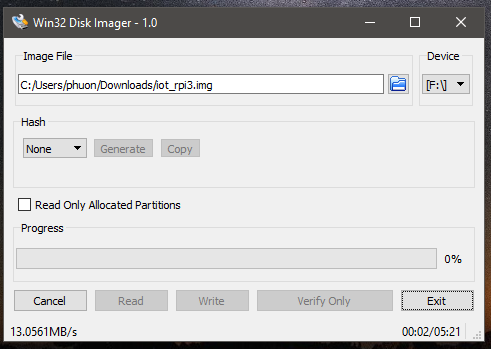
\includegraphics[scale=0.65]{image3/buoc2cach1s13.png}
\end{center}
\caption{Chờ đợi quá trình ghi hệ đièu hành.}
\label{refhinh1}
\end{figure}
\end{center}
\item Sau khi thực hiện quá trình ghi xong, máy tính sẽ hiển thị thông báo yêu cầu định dạng lại thẻ nhớ, ấn "Cancel" để thoát nhé.
\begin{center}
\begin{figure}[htp]
\begin{center}
\includegraphics[scale=0.65]{image3/buoc2cach1s14.png}
\end{center}
\caption{Nhấn Cancel.}
\label{refhinh1}
\end{figure}
\end{center}
\newpage
\item Thông báo của việc ghi hệ điều hành lên thẻ nhớ được thực hiện thành công, nhấn "OK".
\begin{center}
\begin{figure}[htp]
\begin{center}
\includegraphics[scale=0.65]{image3/buoc2cach1s15.png}
\end{center}
\caption{Nhấn OK để tắt thông báo.}
\label{refhinh1}
\end{figure}
\end{center}
\item Vậy là đã cài đặt xong hệ điều hành Android Things lên thẻ nhớ. Việc tiếp theo là gắn thẻ nhớ vào mạch Rpi3.
\begin{center}
\begin{figure}[htp]
\begin{center}
\includegraphics[scale=0.65]{image3/buoc2cach1s16.png}
\end{center}
\caption{Nhấn Exit để thoát chương trình.}
\label{refhinh1}
\end{figure}
\end{center}
\end{enumerate}
\newpage
\hspace*{0.25cm}Cách 2: sử dụng phần mềm \href{https://partner.android.com/things/console/#/tools}{android-things-setup-utility}.
\begin{enumerate}
\item Cắm thẻ nhớ MicroSD vào đầu đọc thẻ, sau đó cắm vào máy tính.
\begin{center}
\begin{figure}[htp]
\begin{center}
\includegraphics[scale=0.8]{image3/buoc2cach1s1.png}
\end{center}
\caption{Nhấn Cancel sau khi cắm thẻ nhớ vô máy.}
\label{refhinh1}
\end{figure}
\end{center}
\item Tải phần mềm từ trang \url{https://partner.android.com/things/console/#/tools}.
\begin{center}
\begin{figure}[htp]
\begin{center}
\includegraphics[scale=0.27]{image3/buoc2cach2s2.png}
\end{center}
\caption{Nhấn DOWNLOAD để tải phần mềm.}
\label{refhinh1}
\end{figure}
\end{center}
\newpage
\item Giải nén phần mềm vừa tải được, chọn tập tin tương ứng với hệ điều hành mà máy tính đang sử dụng.
\begin{center}
\begin{figure}[htp]
\begin{center}
\includegraphics[scale=0.67]{image3/buoc2cach2s3.png}
\end{center}
\caption{Giải nén phần mềm.}
\label{refhinh1}
\end{figure}
\end{center}
\item Chạy tập tin "android-things-setup-utility-windows.exe" (đối với Windows) bằng quyền Administrator. Ấn "YES" nếu có hiện thông báo.
\begin{center}
\begin{figure}[htp]
\begin{center}
\includegraphics[scale=0.57]{image3/buoc2cach2s4.png}
\end{center}
\caption{Chuột phải, chọn Run as administrator.}
\label{refhinh1}
\end{figure}
\end{center}
\item Chọn "1" để tiến hành cài đặt hệ điều hành Android Things.
\begin{center}
\begin{figure}[htp]
\begin{center}
\includegraphics[scale=0.55]{image3/buoc2cach2s5.png}
\end{center}
\caption{Nhấn 1.}
\label{refhinh1}
\end{figure}
\end{center}
\item Chọn "1" để chọn thiết bị phần cứng, ở đây là "Raspberry Pi 3".
\begin{center}
\begin{figure}[htp]
\begin{center}
\includegraphics[scale=0.55]{image3/buoc2cach2s6.png}
\end{center}
\caption{Nhấn 1 để tiếp tục.}
\label{refhinh1}
\end{figure}
\end{center}
\item Sau vài giây để chương trình tiến hành tải công cụ hỗ trợ. Tại đây, có sự 2 lựa chọn phiên bản hệ điều hành để ghi lên thẻ nhớ.
\begin{center}
\begin{figure}[htp]
\begin{center}
\includegraphics[scale=0.55]{image3/buoc2cach2s7.png}
\end{center}
\caption{Lựa chọn phiên bản để ghi.}
\label{refhinh1}
\end{figure}
\end{center}
\begin{itemize}
\item Nếu chưa tạo bản Image Boot và muốn sử dụng bản mặc định thì ấn "1". Đợi từ 10 - 15 phút để tải bản Image Boot.
\begin{center}
\begin{figure}[htp]
\begin{center}
\includegraphics[scale=0.55]{image3/buoc2cach2s8a.png}
\end{center}
\caption{Nhấn 1 nếu cài bản mặc định.}
\label{refhinh1}
\end{figure}
\end{center}
\item Nếu đã tạo (Bước 1) thì ấn "2" để chọn đường dẫn tới tập tin ".zip". Dán địa chỉ của tập tin ".zip" và ấn ENTER.
\begin{center}
\begin{figure}[htp]
\begin{center}
\includegraphics[scale=0.5]{image3/buoc2cach2s8b.png}
\end{center}
\caption{Nhấn 2 để cài bản đã tải tại Bước 1.}
\label{refhinh1}
\end{figure}
\end{center}
\item Dán địa chỉ của tập tin ".zip" và ấn ENTER. Ở đây, địa chỉ là: \textsf{C:/Users/phuon/Downloads/Starter\_Raspberry Pi 3\_1\_New-
Build\_development\_build.zip} rồi ấn "ENTER".
\begin{center}
\begin{figure}[htp]
\begin{center}
\includegraphics[scale=0.5]{image3/buoc2cach2s8c.png}
\end{center}
\caption{Dán địa chỉ chứa tập tin Image Boot .zip.}
\label{refhinh1}
\end{figure}
\end{center}
\end{itemize}
\newpage
\item Sau tải xong công cụ Etcher-cli, ấn ENTER để nhận thẻ nhớ.
\begin{center}
\begin{figure}[htp]
\begin{center}
\includegraphics[scale=0.5]{image3/buoc2cach2s9.png}
\end{center}
\caption{Nhấn ENTER để chọn thẻ nhớ.}
\label{refhinh1}
\end{figure}
\end{center}
\item Nhấn phím mũi tên để chọn thẻ nhớ cần ghi hệ điều hành. Nhấn "ENTER" để xác nhận thẻ nhớ.
\begin{center}
\begin{figure}[htp]
\begin{center}
\includegraphics[scale=0.53]{image3/buoc2cach2s10.png}
\end{center}
\caption{Chọn thẻ nhớ rồi nhấn ENTER.}
\label{refhinh1}
\end{figure}
\end{center}
\newpage
\item Nhấn "y", rồi nhấn "ENTER" để tiếp tục. \textit{Lưu ý, sau khi cài đặt xong sẽ xuất hiện thông báo yêu cầu định dạng lại thẻ nhớ của Windows, ấn "Cancel" nhé!}
\begin{center}
\begin{figure}[htp]
\begin{center}
\includegraphics[scale=0.52]{image3/buoc2cach2s11.png}
\end{center}
\caption{Nhấn y, rồi nhấn ENTER.}
\label{refhinh1}
\end{figure}
\end{center}
\item Đợi khoảng 5 phút thì cài đặt xong. Sau đó ấn "n" để thoát thiết lập mạng.
\begin{center}
\begin{figure}[htp]
\begin{center}
\includegraphics[scale=0.52]{image3/buoc2cach2s12.png}
\end{center}
\caption{Nhấn n rồi nhấn ENTER.}
\label{refhinh1}
\end{figure}
\end{center}
\item Ấn Enter để thoát chương trình.
\begin{center}
\begin{figure}[htp]
\begin{center}
\includegraphics[scale=0.53]{image3/buoc2cach2s13.png}
\end{center}
\caption{Nhấn ENTER để thoát.}
\label{refhinh1}
\end{figure}
\end{center}
\end{enumerate}
\textit{\hspace*{0.25cm}Lưu ý: Sau khi cài hệ điều hành xong, gắn thẻ nhớ vào Rpi3, rồi mới được cắm nguồn. Tuy nhiên nếu có kết nối màn hình HDMI thì nên cắm cáp HDMI trước rồi mới cắm nguồn để tránh trường hợp hình ảnh hiển thị bị sai độ phân giải.}\\

Bước 3: Kết nối mạng cho Raspberry Pi 3 để lấy địa chỉ IP.\\
\hspace*{0.25cm}Cách 1: Kết nối wifi và có màn hình. 
\begin{enumerate}
\item Cắm cáp HDMI với màn hình, gắn bàn phím và chuột vào để điều khiển (nếu màn hình cảm ứng thì không cần thực hiện bước này). Sau đó cắm nguồn cho Rpi3.
\begin{center}
\begin{figure}[htp]
\begin{center}
\includegraphics[scale=0.065]{image3/buoc3s1.JPG}
\end{center}
\caption{Cắm các kết nối trước rồi mới cắm nguồn.}
\label{refhinh1}
\end{figure}
\end{center}
\item Đợi từ 2 - 5 phút cho lần khởi chạy ban đầu, các lần khởi chạy tiếp theo thì thời gian sẽ nhanh hơn.
\begin{center}
\begin{figure}[htp]
\begin{center}
\includegraphics[scale=0.075]{image3/buoc3s2.JPG}
\end{center}
\caption{Chờ hệ điều hành khởi động.}
\label{refhinh1}
\end{figure}
\end{center}
\newpage
\item Tại màn hình chính của Android Things, kéo chuột và nhấp vào phần "Networks".
\begin{center}
\begin{figure}[htp]
\begin{center}
\includegraphics[scale=0.1]{image3/buoc3s3.JPG}
\end{center}
\caption{Chọn Networks.}
\label{refhinh1}
\end{figure}
\end{center}
\item Chọn phần Wi-Fi để kết nối với mạng wifi.
\begin{center}
\begin{figure}[htp]
\begin{center}
\includegraphics[scale=0.15]{image3/buoc3s4.JPG}
\end{center}
\caption{Chọn Wi-Fi.}
\label{refhinh1}
\end{figure}
\end{center}
\item Nếu mới lần đầu kết nối, thì sẽ hiện chữ "Off". Để bật wifi, ấn vào nút cùng hàng với "Off" ở phía bên phải màn hình.
\begin{center}
\begin{figure}[htp]
\begin{center}
\includegraphics[scale=0.12]{image3/buoc3s5.JPG}
\end{center}
\caption{Ấn nút bên phải để bật wifi.}
\label{refhinh1}
\end{figure}
\end{center}
\newpage
\item Sau khi bật wifi, danh sách các wifi khả dụng sẽ được hiện ra.
\begin{center}
\begin{figure}[htp]
\begin{center}
\includegraphics[scale=0.12]{image3/buoc3s6.JPG}
\end{center}
\caption{Danh sách wifi khả dụng.}
\label{refhinh1}
\end{figure}
\end{center}
\item Chọn wifi, và nhập vào mật khẩu của wifi mà muốn thiết bị kết nối. Nhấn "CONNECT".
\begin{center}
\begin{figure}[htp]
\begin{center}
\includegraphics[scale=0.12]{image3/buoc3s7.JPG}
\end{center}
\caption{Nhập mật khẩu và nhấn CONNECT.}
\label{refhinh1}
\end{figure}
\end{center}
\item Nếu thấy hiện chữ "Connected", tức là đã kết nối wifi thành công. Ấn dấu mũi tên \b{<} để quay lại màn hình chính, địa chỉ của thiết bị sẽ được hiện ra. Ở đây là: "192.168.2.55".
\begin{center}
\begin{figure}[htp]
\begin{center}
\includegraphics[scale=0.15]{image3/buoc3s8.JPG}
\end{center}
\caption{Nhấn < để về màn hình chính.}
\label{refhinh1}
\end{figure}
\end{center}
\newpage
\item Địa chỉ IP của thiết bị sẽ được hiện ra trong phần "Networks". Ở đây là: "192.168.2.55".
\begin{center}
\begin{figure}[htp]
\begin{center}
\includegraphics[scale=0.17]{image3/buoc3s9.JPG}
\end{center}
\caption{Networks hiển thị IP của mạch Rpi3.}
\label{refhinh1}
\end{figure}
\end{center}
\end{enumerate}
\hspace*{0.25cm}Cách 2: Kết nối mạng dây và không có màn hình. 
\begin{enumerate}
\item Cắm cáp Ethernet vào mạch Rpi3, sau đó cắm nguồn.
\begin{center}
\begin{figure}[htp]
\begin{center}
\includegraphics[scale=0.08]{image3/buoc3s10.JPG}
\end{center}
\caption{Cắm dây Ethernet và cắm nguồn.}
\label{refhinh1}
\end{figure}
\end{center}
\item Đợi từ 2 - 5 phút cho lần khởi chạy ban đầu, các lần khởi chạy tiếp theo thì thời gian sẽ nhanh hơn.
\item Kết nối laptop/desktop cùng với mạng đã kết nối với Rpi3. Sử dụng phần mềm \hyperref[scanip]{Advanced IP Scanner}, tìm với tên tại cột "Nhà sản xuất" là "Raspberry Pi Fundation" để lấy địa chỉ IP (192.168.2.55).
\begin{center}
\begin{figure}[htp]
\begin{center}
\includegraphics[scale=0.65]{image3/buoc3s11.png}
\end{center}
\caption{Chạy chương trình \hyperref[scanip]{Advanced IP Scanner} để quét địa chỉ IP của Rpi3.}
\label{refhinh1}
\end{figure}
\end{center}
\end{enumerate}
Bước 4: Kết nối với Raspberry Pi 3 bằng địa chỉ IP.
\begin{enumerate}
\item Sau khi có được địa chỉ của mạch Rpi3. Chạy ứng dụng \hyperref[ADB]{ADB} để thực hiện việc kết nối.
\begin{center}
\begin{figure}[htp]
\begin{center}
\includegraphics[scale=0.62]{image3/buoc3s12.png}
\end{center}
\caption{Truy cập thư mục platform-tools.}
\end{figure}
\end{center}
\item Chạy "Command Prompt" (Windows) hoặc "Terminal" (Mac/Linux), tại thư mục (platform-tools) chứa tập tin "adb".
\begin{center}
\begin{figure}[htp]
\begin{center}
\includegraphics[scale=0.6]{image3/buoc3s13.png}
\end{center}
\caption{Chạy Command Prompt tại thư mục platform-tools.}
\end{figure}
\end{center}
\item Nhập lệnh "adb connect <IP>", với <IP> là địa chỉ IP của mạch Rpi3. Ví dụ "adv connect 192.68.2.55".
\begin{center}
\begin{figure}[htp]
\begin{center}
\includegraphics[scale=0.55]{image3/buoc3s14.png}
\end{center}
\caption{Kết nối với thiết bị "adb connect <IP>".}
\label{refhinh1}
\end{figure}
\end{center}
\newpage
\item Kết nối thành công với địa chỉ IP 192.168.2.55 thông qua port 5555.
\begin{center}
\begin{figure}[htp]
\begin{center}
\includegraphics[scale=0.65]{image3/buoc3s15.png}
\end{center}
\caption{Kết nối với mạch Raspberry Pi 3 thành công.}
\label{refhinh1}
\end{figure}
\end{center}
\item Nếu muốn huỷ kết nối với một thiết bị thì dùng lệnh "adb disconnect <IP>.
\begin{center}
\begin{figure}[htp]
\begin{center}
\includegraphics[scale=0.6]{image3/buoc3s16.png}
\end{center}
\caption{Hủy kết nối với một thiết bị "adb disconnect <IP>".}
\end{figure}
\end{center}
\item Còn nếu muốn huỷ hết các thiết bị đang kết nối thì nhập lệnh "adb disconnect".
\begin{center}
\begin{figure}[htp]
\begin{center}
\includegraphics[scale=0.6]{image3/buoc3s17.png}
\end{center}
\caption{Hủy kết nối với tất cả thiết bị "adb disconnect".}
\end{figure}
\end{center}
\end{enumerate}
\newpage
\subsection{Các công cụ hỗ trợ}
\subsubsection{Thay đổi hình ảnh của Image Boot}
\label{bootanimation}
Để thay đổi hình ảnh của Image Boot khi chạy hệ điều hành Android Things, thì phải sử dụng tập tin "bootanimation.zip" tại bước tạo Image Boot.\\
Phần hướng dẫn về cách tạo "bootadnimation.zip" hoặc có thể tải các tập tin bootanimation.zip từ trên mạng:

\begin{enumerate}
\item Chọn một đoạn clip từ 5 - 10 giây.
\item Sử dụng công cụ DVDVideoSoft Free Studio để tách đoạn clip thành hình ảnh.
\item Chia ảnh vào các thư mục phù hợp.
\item Dùng công cụ Boot Animation Creator để tạo ra file "bootanimation.zip".
\item Tại \hyperref[truong4]{trường "4"}, nhấn "UPLOAD" để tải lên tập tin "bootanimation.zip".

\begin{center}
\begin{figure}[htp]
\begin{center}
\includegraphics[scale=0.5]{image3/sat11.png}
\end{center}
\caption{Chọn UPLOAD.}
\end{figure}
\end{center}
\item Hiện lên thông báo "Upload a build resource", nhấn chọn biểu tượng thư mục.
\begin{center}
\begin{figure}[htp]
\begin{center}
\includegraphics[scale=0.5]{image3/sat21.png}
\end{center}
\caption{Chọn biểu tượng thư mục.}
\end{figure}
\end{center}
\item Chọn tập tin "bootanimation.zip" cần tải lên.
\begin{center}
\begin{figure}[htp]
\begin{center}
\includegraphics[scale=0.5]{image3/sat22.png}
\end{center}
\caption{Chọn file "bootanimation.zip", nhấn OK.}
\end{figure}
\end{center}
\item Tập tin được tải lên thành công, sau đó ấn "NEXT" để tiếp tục \hyperref[truong5]{trường "5"}.
\begin{center}
\begin{figure}[htp]
\begin{center}
\includegraphics[scale=0.5]{image3/sat23.png}
\end{center}
\caption{Tải tập tin thành công, ấn NEXT để \hyperref[truong5]{tiếp tục}.}
\end{figure}
\end{center}
\end{enumerate}
\newpage
\subsubsection{Advanced IP Scanner (Windows)}
\label{scanip}
\href{https://www.advanced-ip-scanner.com/}{Advanced IP Scanner} là ứng dụng quét mạng miễn phí, hoạt động nhanh và rất dễ sử dụng dành cho người dùng Windows. Chỉ trong vài giây, công cụ này sẽ tìm ra tất cả các máy trong mạng và cung cấp cách truy cập dễ dàng vào các nguồn tài nguyên của chúng, ví dụ như HTTP, HTTPS, FTP hoặc folder đã chia sẻ. Với Advanced IP Scanner, người dùng có thể bật và tắt máy từ xa.
\begin{itemize}
\item Tải \href{https://www.advanced-ip-scanner.com/}{tại đây}: \url{https://www.advanced-ip-scanner.com/}
\item Hướng dẫn sử dụng:
\begin{enumerate}
\item Chạy "Command Prompt" (Windows) nhập lệnh "ipconfig" hoặc "Terminal" (Mac/Linux) nhập lệnh "ifconfig" để lấy địa chỉ IPv4 hiện tại.
\begin{center}
\begin{figure}[htp]
\begin{center}
\includegraphics[scale=0.5]{image3/ipconfig.jpg}
\end{center}
\caption{Lệnh "ipconfig" trên Windows.}
\label{refhinh1}
\end{figure}
\end{center}
\begin{center}
\begin{figure}[htp]
\begin{center}
\includegraphics[scale=0.6]{image3/ifconfig.png}
\end{center}
\caption{Lệnh "ifconfig" trên Mac/Linux.}
\label{refhinh1}
\end{figure}
\end{center}
\newpage
\item Nhập khoảng địa chỉ mà máy tính đang kết nối để quét. Ví dụ: IP máy tính 192.168.0.30, thì sẽ nhập khoảng 192.168.0.1 - 192.168.0.254. 
\item Sau đó ấn "Scan". Kết quả sau khi quét sẽ được trả về như \hyperref[ips]{hình \ref*{ips}}.
\begin{center}
\begin{figure}[htp]
\begin{center}
\includegraphics[scale=0.6]{image3/ipscanner.png}
\end{center}
\caption{Nhấn Scan để quét.}
\label{ips}
\end{figure}
\end{center}
\end{enumerate}
\end{itemize}
 
 \subsubsection{ADB}
 \label{ADB}ADB thường được sử dụng khi cố gắng chạy các ứng dụng dành cho điện thoại trên máy tính, do đó bạn có thể debug (gỡ lỗi) các lỗi trên các ứng dụng của mình, ứng dụng mà bạn đang tạo. ADB được sử dụng cho các thiết bị Android root.\\
 Lý do bởi vì ADB cho phép bạn giao tiếp với một điện thoại Android ở mức độ phát triển nào đó, do đó nó rất tiện dụng trong một số trường hợp chẳng hạn như khi chúng ta muốn ra lệnh cho phép mình chuyển các tập tin vào thiết bị và sau đó thực thi tất cả các tập tin trong điện thoại đã root.\\
 Cài đặt ADB:
 \begin{enumerate}
     \item vào trang wed này để tải ADB:  \url{https://forum.xda-developers.com/showthread.php?p=48915118#post48915118}
 \begin{center}
    \begin{figure}[htp]
    \begin{center}
     \includegraphics[scale=0.35]{image3/adb1}
    \end{center}
    \caption{Tệp adb được tải về.}
    \label{refhinh1}
    \end{figure}
\end{center}
    \item Chạy file adb vừa tải về. sau đó nhấn Y để cài đặt.
\newpage
 \begin{center}
    \begin{figure}[htp]
    \begin{center}
     \includegraphics[scale=0.35]{image3/giaodienadb}
    \end{center}
    \caption{Giao diện adb.}
    \label{refhinh1}
    \end{figure}
\end{center}
 \end{enumerate}
 
 \subsection{Project LED Blinky}
 Chuẩn bị:\\
 - 1 board raspberry pi 3.\\
 - 1 điện trở 200 Ohm\\
 - 1 led.\\
 - 1 breadboard.\\
 \newline
 Thực hiện nối mạch như hình.
 \begin{center}
    \begin{figure}[htp]
    \begin{center}
     \includegraphics[scale=0.35]{image3/blinkled}
    \end{center}
    \caption{Mạch blink led.}
    \label{refhinh1}
    \end{figure}
\end{center}
\newpage
Vào trang web \url{https://github.com/HungSoma/Android-Things-vs-Raspberry-PI-3?fbclid=IwAR0tdUJqoOSLQh-S8M65RqXznjtD_5BN9wdSy-MtYrcwdeIticqTMrJ4bVc}.\\

Mở android studio, mở project blink led, màn hình xuất hiện như sau.
 \begin{center}
    \begin{figure}[htp]
    \begin{center}
     \includegraphics[scale=0.3]{image3/androidblinkled}
    \end{center}
    \caption{Giao diện android.}
    \label{refhinh1}
    \end{figure}
\end{center}

Bạn xem địa chỉ IP của raspberry, ở đây của mình là 192.168.2.18
\begin{center}
    \begin{figure}[htp]
    \begin{center}
     \includegraphics[scale=0.15]{image3/ip.jpg}
    \end{center}
    \caption{IP raspberry.}
    \label{refhinh1}
    \end{figure}
\end{center}
 
 Mở Command Prompt sau đó gõ lenh adb để khởi động adb.
\newpage
\begin{center}
    \begin{figure}[htp]
    \begin{center}
     \includegraphics[scale=0.5]{image3/ADB}
    \end{center}
    \caption{Gõ lệnh adb.}
    \label{refhinh1}
    \end{figure}
\end{center}

Tiếp tục gõ lệnh: abc connect 192.168.2.18 để kêt nối, 192.168.2.18 là địa chỉ ip hiện tại của mình, các bạn hay thay địa chỉ ip của các bạn.\\
Kích vào nút run app trên android studio để xem kết nối.Sau đó nhân ok để nạp.
\begin{center}
    \begin{figure}[htp]
    \begin{center}
     \includegraphics[scale=0.5]{image3/adbketnoi}
    \end{center}
    \caption{Kết nối PC với raspberry.}
    \label{refhinh1}
    \end{figure}
\end{center}
\newpage
\begin{center}
    \begin{figure}[htp]
    \begin{center}
     \includegraphics[scale=0.5]{image3/androidketnoi}
    \end{center}
    \caption{Hiển thị kết nối trên androidstudio.}
    \label{refhinh1}
    \end{figure}
\end{center}

\begin{center}
    \begin{figure}[htp]
    \begin{center}
     \includegraphics[scale=0.25]{image3/ketqua.jpg}
    \end{center}
    \caption{Kết quả hiển thị trên raspberry.}
    \label{refhinh1}
    \end{figure}
\end{center}
